\documentclass[11pt, a4paper]{article}

% Packages
\usepackage[margin=2.2cm]{geometry}
\usepackage{fontenc}
\usepackage{inputenc}
\usepackage{microtype}
\usepackage{graphicx}
\usepackage{booktabs}
\usepackage{tabularx}
\usepackage{caption}
\usepackage{subcaption}
\usepackage{float}
\usepackage{amsmath}
\usepackage{hyperref}
\usepackage{parskip}
\usepackage{titlesec}
\usepackage{fancyhdr}
\usepackage{enumitem}
\usepackage{xcolor}


% Minimal black styling
\hypersetup{colorlinks=false, pdfborder={0 0 0}}
\definecolor{lightgray}{gray}{0.92}

% Title formatting: bold sections, no extra spacing
\titleformat{\section}{\large\bfseries}{}{0em}{}[\titlerule]
\titleformat{\subsection}{\normalsize\bfseries}{}{0em}{}
\titleformat{\subsubsection}{\normalsize\itshape}{}{0em}{}
\titlespacing{\section}{0pt}{14pt}{6pt}
\titlespacing{\subsection}{0pt}{10pt}{4pt}

% Header/footer
\pagestyle{fancy}
\fancyhf{}
\fancyhead[L]{\small Individual Project}
\fancyhead[R]{\small Manya Jain | 2024102068}
\fancyfoot[C]{\thepage}
\renewcommand{\headrulewidth}{0.4pt}

% Tighter lists
\setlist{nosep, topsep=2pt}

\begin{document}

% ---- TITLE PAGE ----
\begin{titlepage}
  \centering
  \vspace*{3cm}
  {\Large\bfseries Individual Project\par}
  \vspace{0.5cm}
  {\large Language Model Architecture\par}
  \vspace{2cm}
  {\large Manya Jain\par}
  {\normalsize 2024102068\par}
  \vspace{0.5cm}
  {\normalsize IIIT Hyderabad\par}
  \vfill
  {\normalsize September 2026\par}
\end{titlepage}

% ---- TABLE OF CONTENTS ----
\tableofcontents
\newpage

% ===========================================================================
\section{Phase 1: Tokenizer Training}

The first phase was about building tokenizers from scratch for two languages: Hindi (Model H, the higher-resource model) and Nepali (Model L, the lower-resource model). The goal was to train byte-pair encoding (BPE) tokenizers directly on raw text scraped from online sources, without using any pretrained vocabulary.

\subsection{Data Collection}

Getting enough Nepali text was genuinely the hard part here. Hindi has OSCAR, Wikipedia dumps, and plenty of news data readily available. Nepali required pulling from smaller sources like news archives and OCR-processed documents to get a comparable volume. The quality was also lower since OCR introduces noise.

\subsection{Tokenizer Configuration}

Both tokenizers were trained using the HuggingFace \texttt{tokenizers} library with BPE, Unicode normalization, and no pre-tokenization (character-level splits before BPE). Final vocabulary sizes were chosen to balance coverage vs. unknown-token rate.

\begin{table}[H]
\centering
\caption{Tokenizer Summary}
\begin{tabular}{lcc}
\toprule
\textbf{Property} & \textbf{Model H (Hindi)} & \textbf{Model L (Nepali)} \\
\midrule
Vocabulary Size & 16,000 & 16,240 \\
Avg. Bytes per Token & 10.31 & 13.16 \\
Script & Devanagari & Devanagari \\
\bottomrule
\end{tabular}
\end{table}

The Nepali tokenizer ends up with a higher bytes-per-token ratio (13.16 vs 10.31), meaning it packs more information into each token. This is efficient for compression but means the model needs to attend further back in context to cover the same semantic span. This difference shows up later in the BPB evaluation numbers.

% ===========================================================================
\section{Phase 2: Pretraining}

\subsection{Architecture}

Both models are decoder-only Transformers (GPT-style) built entirely from scratch in PyTorch. No use of \texttt{nn.Transformer} or HuggingFace model classes. Everything including the multi-head attention, positional embeddings, and the causal mask was written manually.

The attention formula used is:
\[
  \text{Attention}(Q,K,V) = \text{softmax}\!\left(\frac{QK^\top}{\sqrt{d_k}} + M\right) V
\]
where $M$ is a causal upper-triangular mask filled with $-\infty$ to prevent attending to future tokens.

\begin{table}[H]
\centering
\caption{Model Architecture Configuration}
\begin{tabular}{lcc}
\toprule
\textbf{Parameter} & \textbf{Model H (Hindi)} & \textbf{Model L (Nepali)} \\
\midrule
Hidden Dim ($d_{model}$) & 512 & 512 \\
Attention Heads & 8 ($d_k = 64$) & 8 ($d_k = 64$) \\
Layers & 6 & 6 \\
Feed-Forward Dim & 1,536 & 1,536 \\
Context Length & 512 & 512 \\
Dropout & 0.1 & 0.1 \\
Trainable Parameters & \textbf{24.22M} & \textbf{24.34M} \\
\bottomrule
\end{tabular}
\end{table}

Key design choices:
\begin{itemize}
  \item \textbf{Pre-LayerNorm}: LayerNorm applied before each sublayer (more stable training than Post-LN).
  \item \textbf{Weight Tying}: The output projection is tied to the input embedding matrix, which cuts down parameters and regularizes the output space.
  \item \textbf{GELU activations} in the feed-forward sublayer.
  \item \textbf{Learned positional embeddings} via \texttt{nn.Embedding(context\_len, d\_model)}.
\end{itemize}

\subsection{Training Setup}

Both models were trained for 61,036 steps using AdamW with cosine learning rate scheduling (with warmup). Checkpoints were saved with full optimizer and scheduler states so training could be resumed cleanly.

\subsection{Loss Curves}

\begin{figure}[H]
\centering
\begin{subfigure}[b]{0.48\textwidth}
  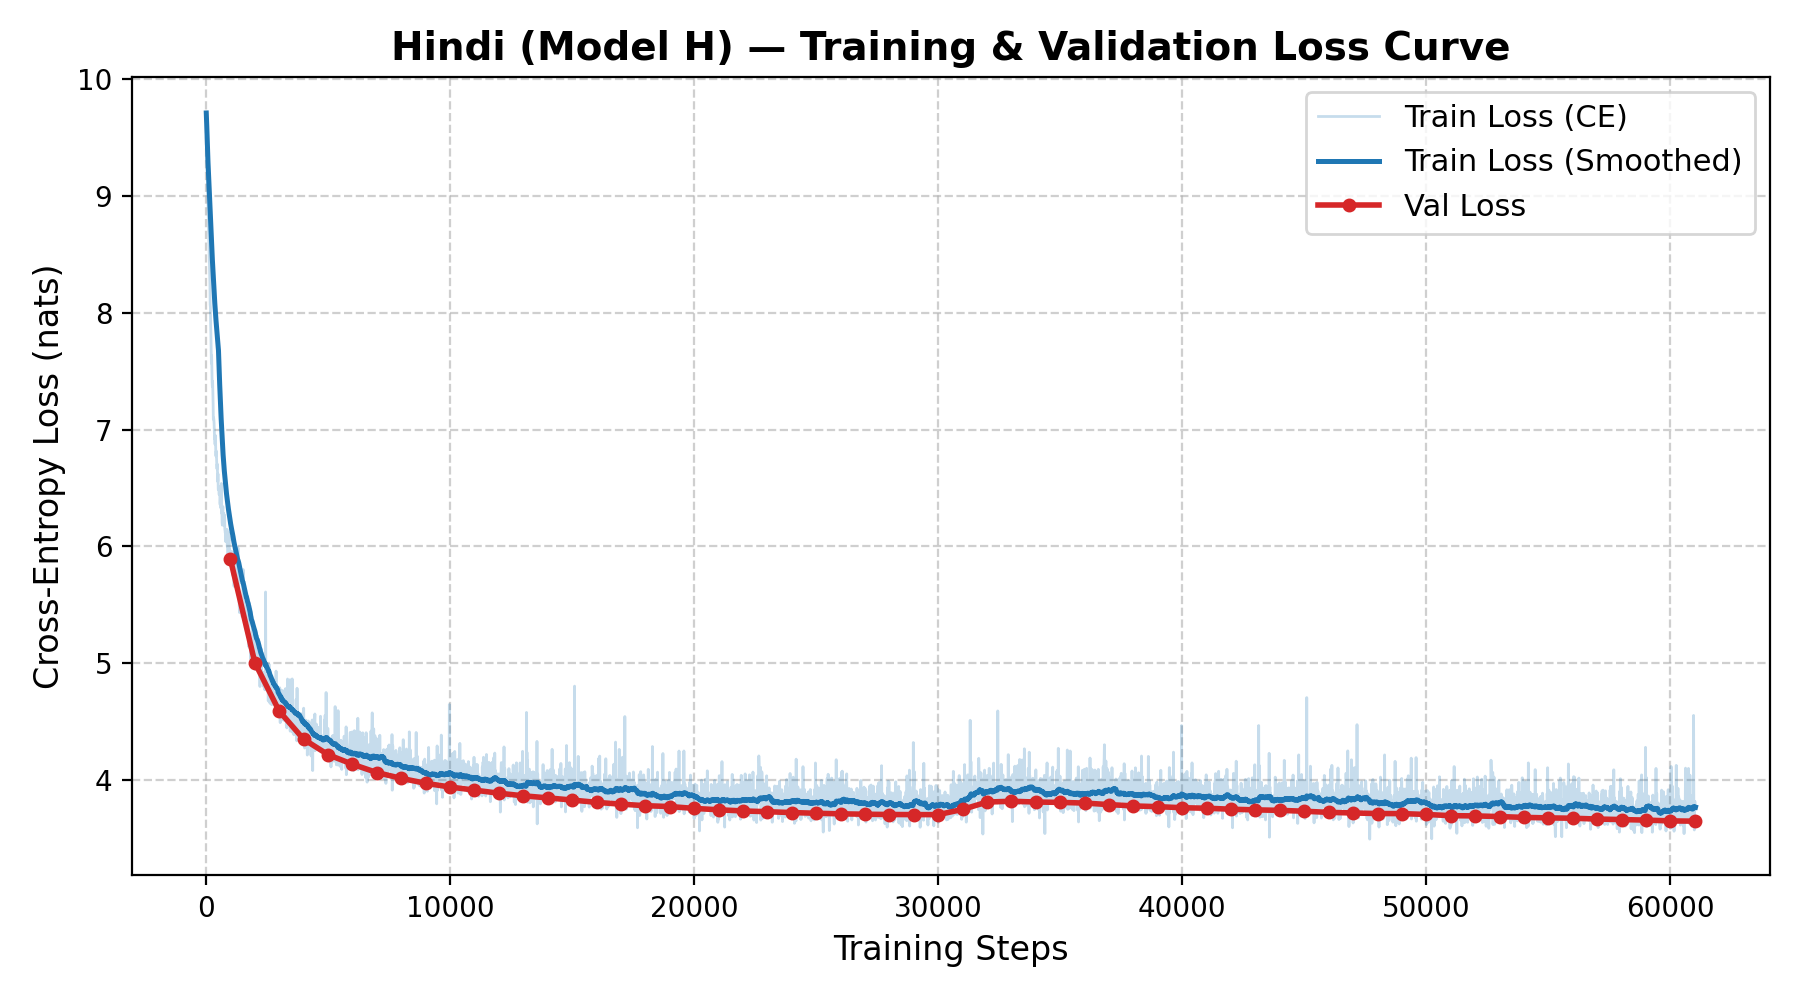
\includegraphics[width=\textwidth]{plots/phase2_hindi_loss_curve.png}
  \caption{Hindi (Model H) Training Loss}
\end{subfigure}
\hfill
\begin{subfigure}[b]{0.48\textwidth}
  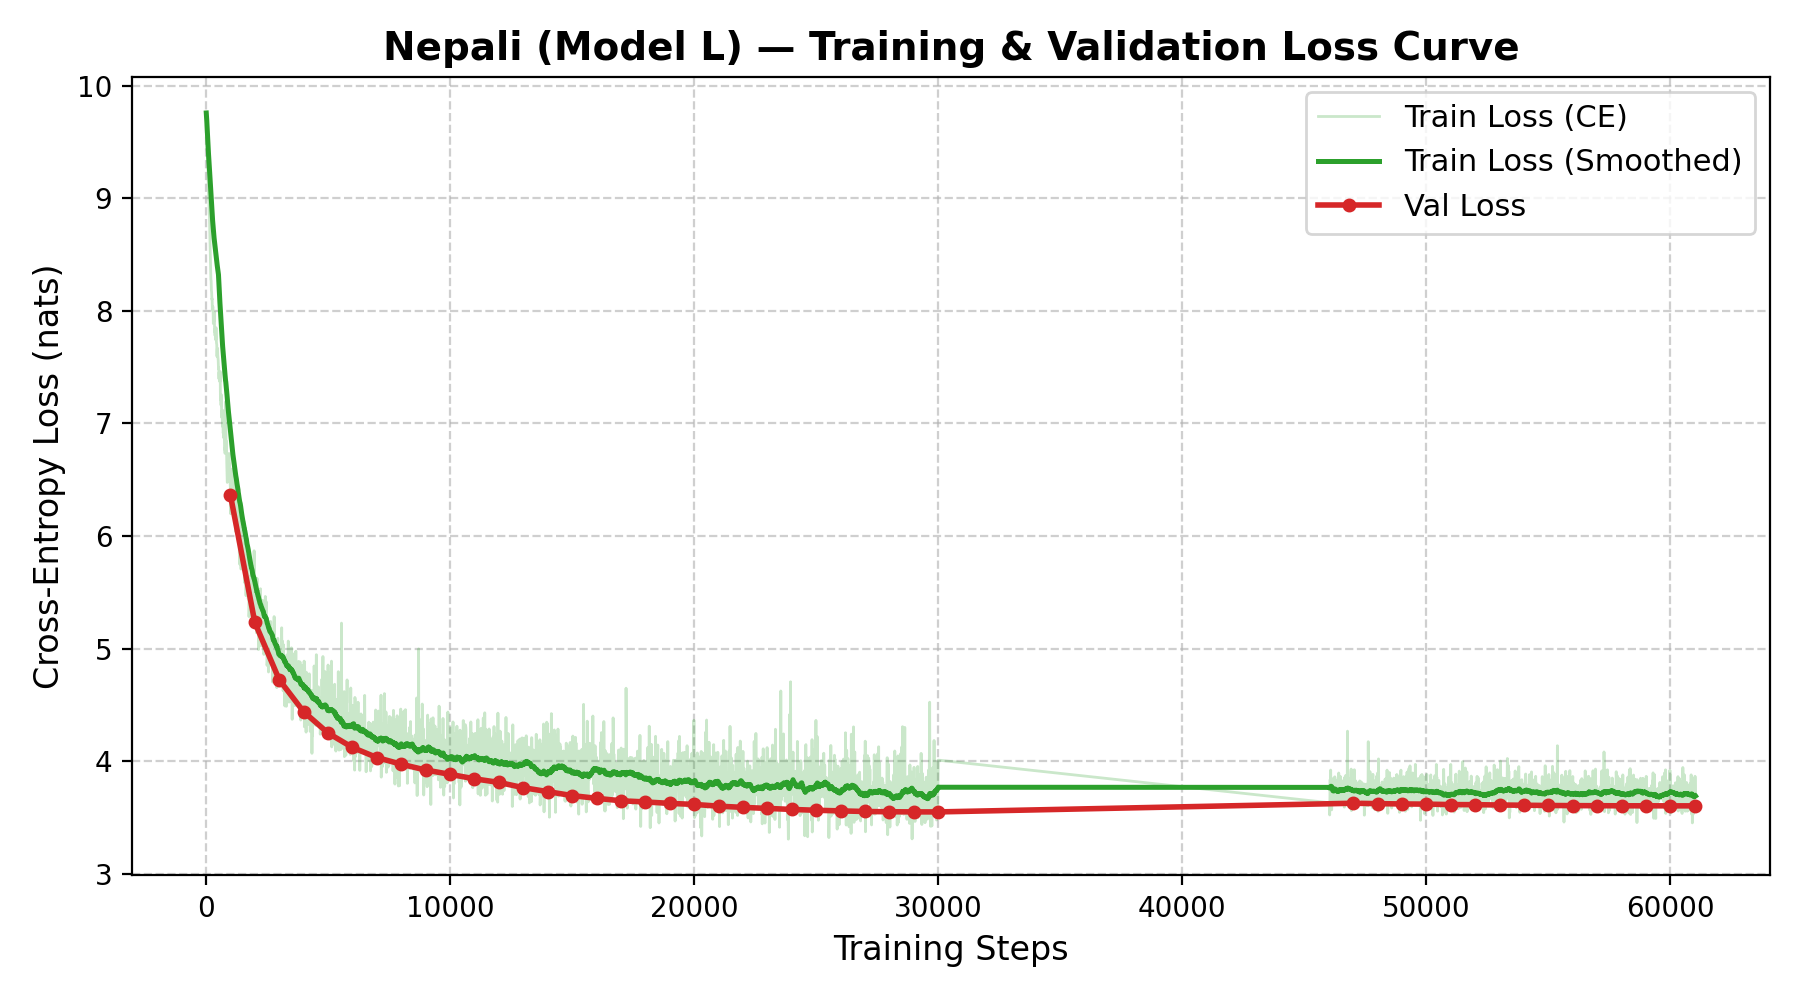
\includegraphics[width=\textwidth]{plots/phase2_nepali_loss_curve.png}
  \caption{Nepali (Model L) Training Loss}
\end{subfigure}
\caption{Training and validation loss curves for both models across pretraining.}
\end{figure}

\begin{figure}[H]
\centering
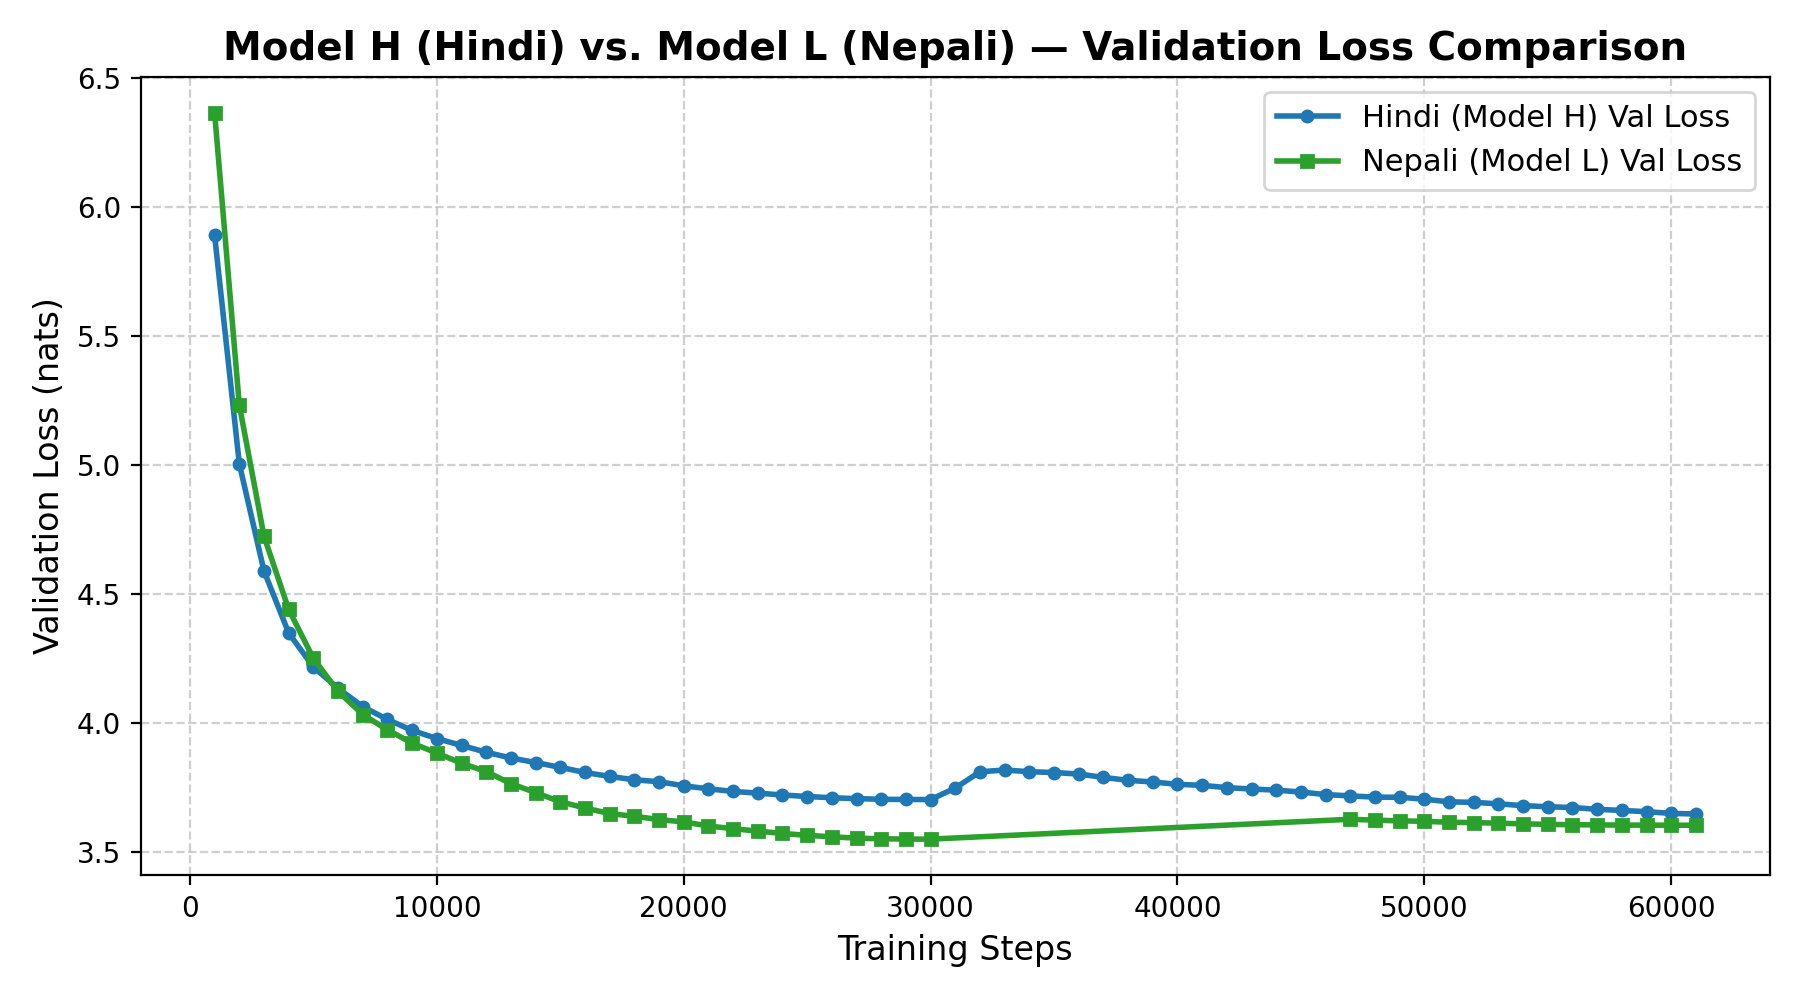
\includegraphics[width=0.72\textwidth]{plots/phase2_comparison_loss_curve.png}
\caption{Side-by-side validation loss comparison. Both models converge smoothly, with Nepali reaching slightly lower absolute loss.}
\end{figure}

\subsection{Intrinsic Evaluation Metrics}

\begin{table}[H]
\centering
\caption{Language Modeling Metrics on Held-Out Test Set}
\begin{tabular}{lccc}
\toprule
\textbf{Metric} & \textbf{Model H (Hindi)} & \textbf{Model L (Nepali)} & \textbf{Note} \\
\midrule
Validation Loss (nats) & 3.6487 & 3.5910 & Cross-entropy \\
Test Loss (nats) & 3.6663 & 3.5923 & Cross-entropy \\
Perplexity (PPL) & 39.11 & 36.32 & $e^{\text{Loss}}$ \\
Bits-Per-Byte (BPB) & 0.5131 & 0.3939 & Normalized for tokenizer \\
\bottomrule
\end{tabular}
\end{table}

Nepali beats Hindi on both PPL and BPB. The lower BPB (0.39 vs 0.51) is largely explained by the tokenizer difference: Nepali tokens carry more bytes on average, so there are fewer tokens to predict per unit of text, making the per-token cross-entropy translate to a lower per-byte cost. Both numbers indicate healthy convergence.

\subsection{Generation Quality}

Continuations were evaluated under greedy decoding and temperature sampling at 0.5, 1.0, and 1.5.

\begin{table}[H]
\centering
\caption{Generation Quality Metrics}
\small
\begin{tabular}{llccc}
\toprule
\textbf{Decoding} & \textbf{Model} & \textbf{BLEU-4} & \textbf{chrF} & \textbf{ROUGE-L} \\
\midrule
Greedy & Hindi  & 0.9488 & 12.21 & 0.1243 \\
       & Nepali & 1.2197 & 13.54 & 0.0838 \\
Temp 0.5 & Hindi  & 0.7732 & 13.45 & 0.0921 \\
         & Nepali & 1.5608 & 19.88 & 0.0966 \\
Temp 1.0 & Hindi  & 0.7182 & 12.71 & 0.0906 \\
         & Nepali & 1.0644 & 19.27 & 0.0901 \\
\bottomrule
\end{tabular}
\end{table}

\begin{table}[H]
\centering
\caption{Fluency and Diversity Diagnostics}
\small
\begin{tabular}{llccc}
\toprule
\textbf{Decoding} & \textbf{Model} & \textbf{4-gram Rep.} & \textbf{Distinct-1} & \textbf{Distinct-2} \\
\midrule
Greedy   & Hindi  & 0.2659 & 0.4270 & 0.6215 \\
         & Nepali & 0.6712 & 0.2291 & 0.3167 \\
Temp 0.5 & Hindi  & 0.1012 & 0.4605 & 0.7336 \\
         & Nepali & 0.3351 & 0.3981 & 0.6283 \\
Temp 1.0 & Hindi  & 0.0267 & 0.6838 & 0.9313 \\
         & Nepali & 0.0213 & 0.7214 & 0.9586 \\
Temp 1.5 & Hindi  & 0.0000 & 0.9447 & 1.0000 \\
         & Nepali & 0.0000 & 0.9079 & 0.9990 \\
\bottomrule
\end{tabular}
\end{table}

The Nepali greedy repetition rate (67.12\%) is much worse than Hindi (26.59\%). This makes sense given the narrower corpus: with less training diversity, the model learns to fall back on the same token patterns more aggressively. Sampling at temperature 1.0 fixes this completely for both models (repetition drops to near 0\%).

\subsection{Attention Analysis (Phase 2)}

Attention heatmaps were extracted at Layer 0 (early), Layer 3 (middle), and Layer 5 (late).

\begin{figure}[H]
\centering
\begin{subfigure}[b]{0.31\textwidth}
  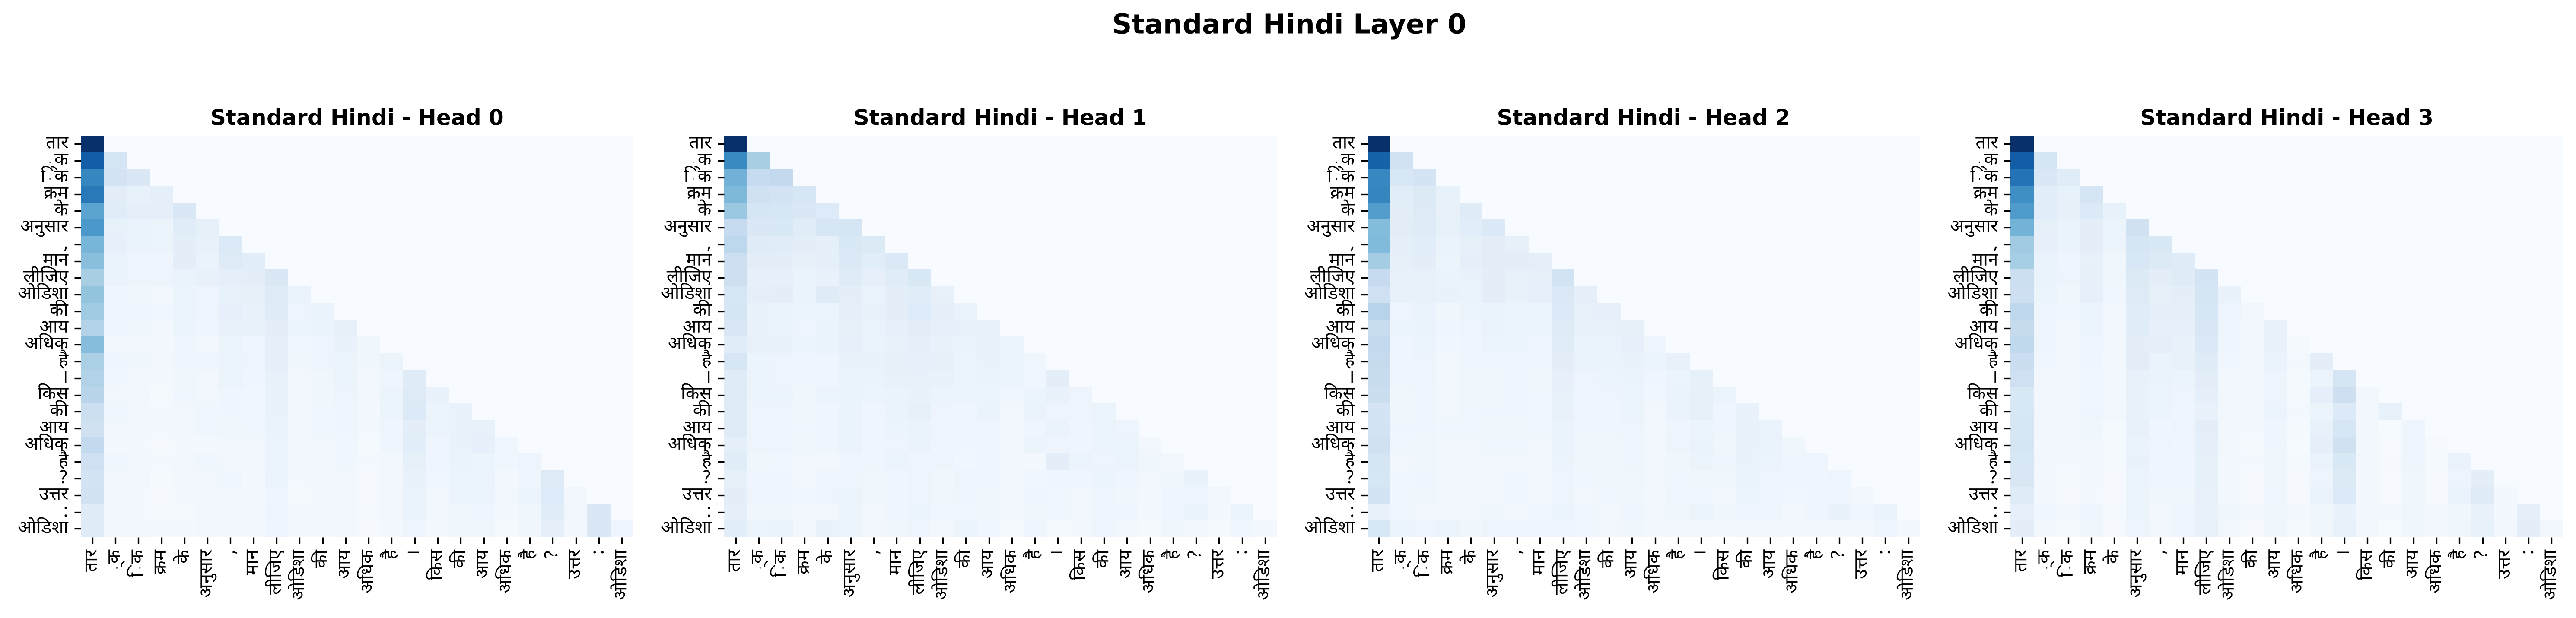
\includegraphics[width=\textwidth]{plots/phase2_hindi_attn_layer0.png}
  \caption{Hindi Layer 0}
\end{subfigure}
\hfill
\begin{subfigure}[b]{0.31\textwidth}
  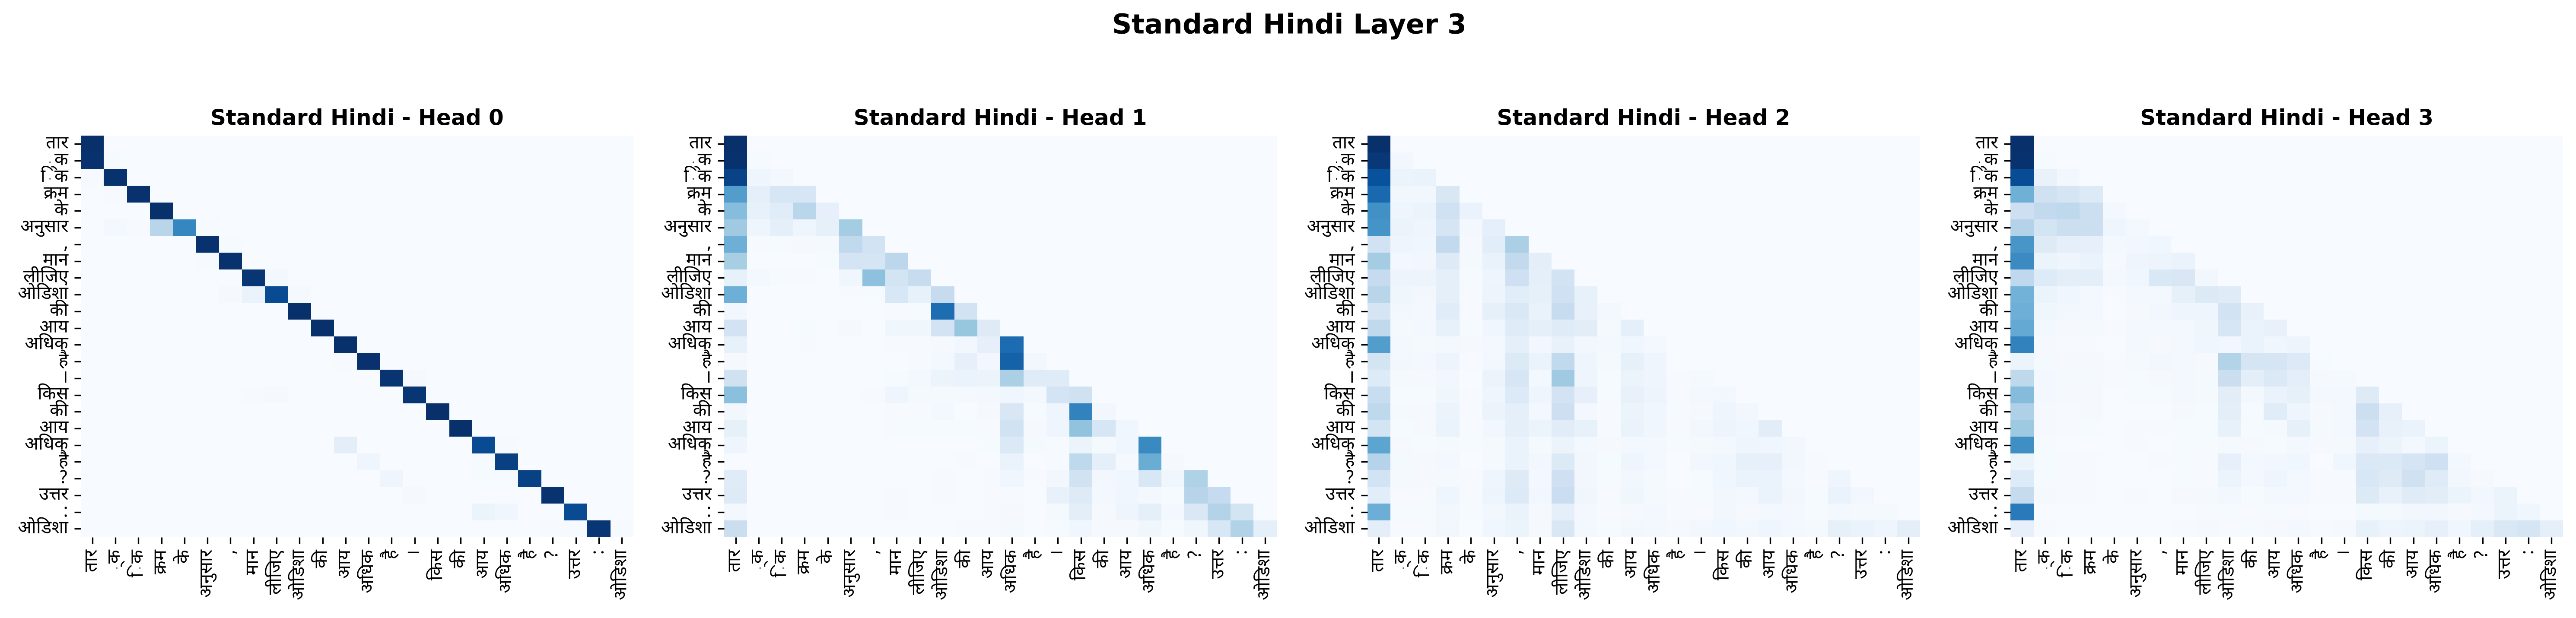
\includegraphics[width=\textwidth]{plots/phase2_hindi_attn_layer3.png}
  \caption{Hindi Layer 3}
\end{subfigure}
\hfill
\begin{subfigure}[b]{0.31\textwidth}
  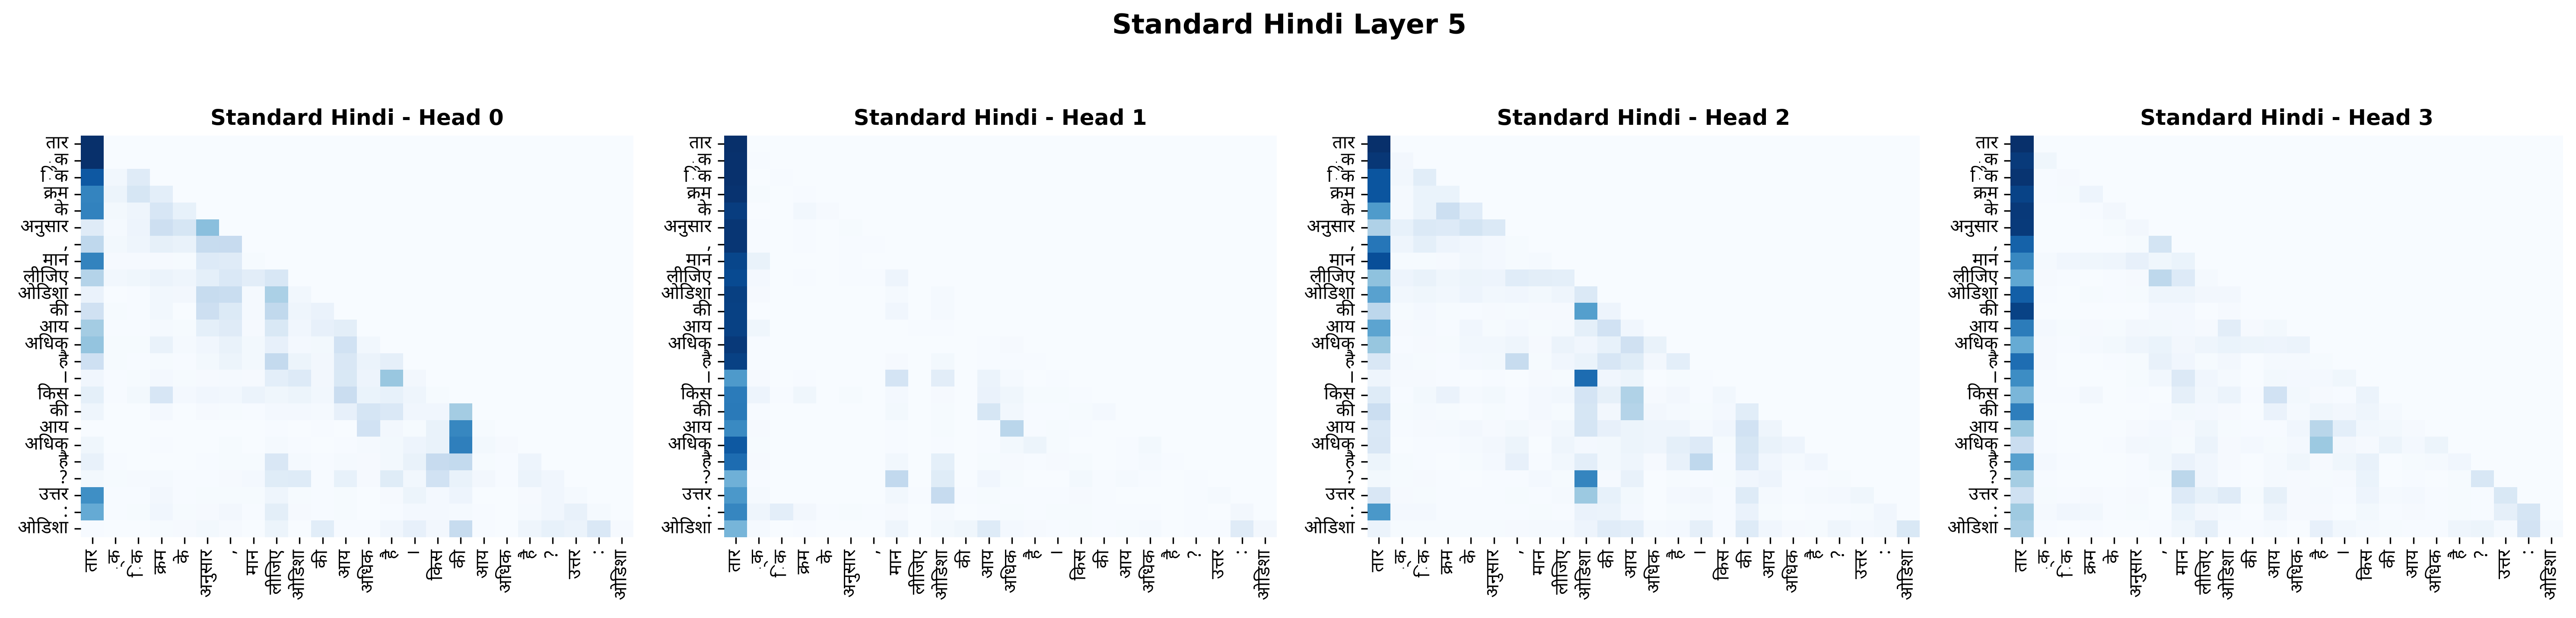
\includegraphics[width=\textwidth]{plots/phase2_hindi_attn_layer5.png}
  \caption{Hindi Layer 5}
\end{subfigure}
\caption{Hindi pretrained attention heatmaps across layers.}
\end{figure}

\begin{figure}[H]
\centering
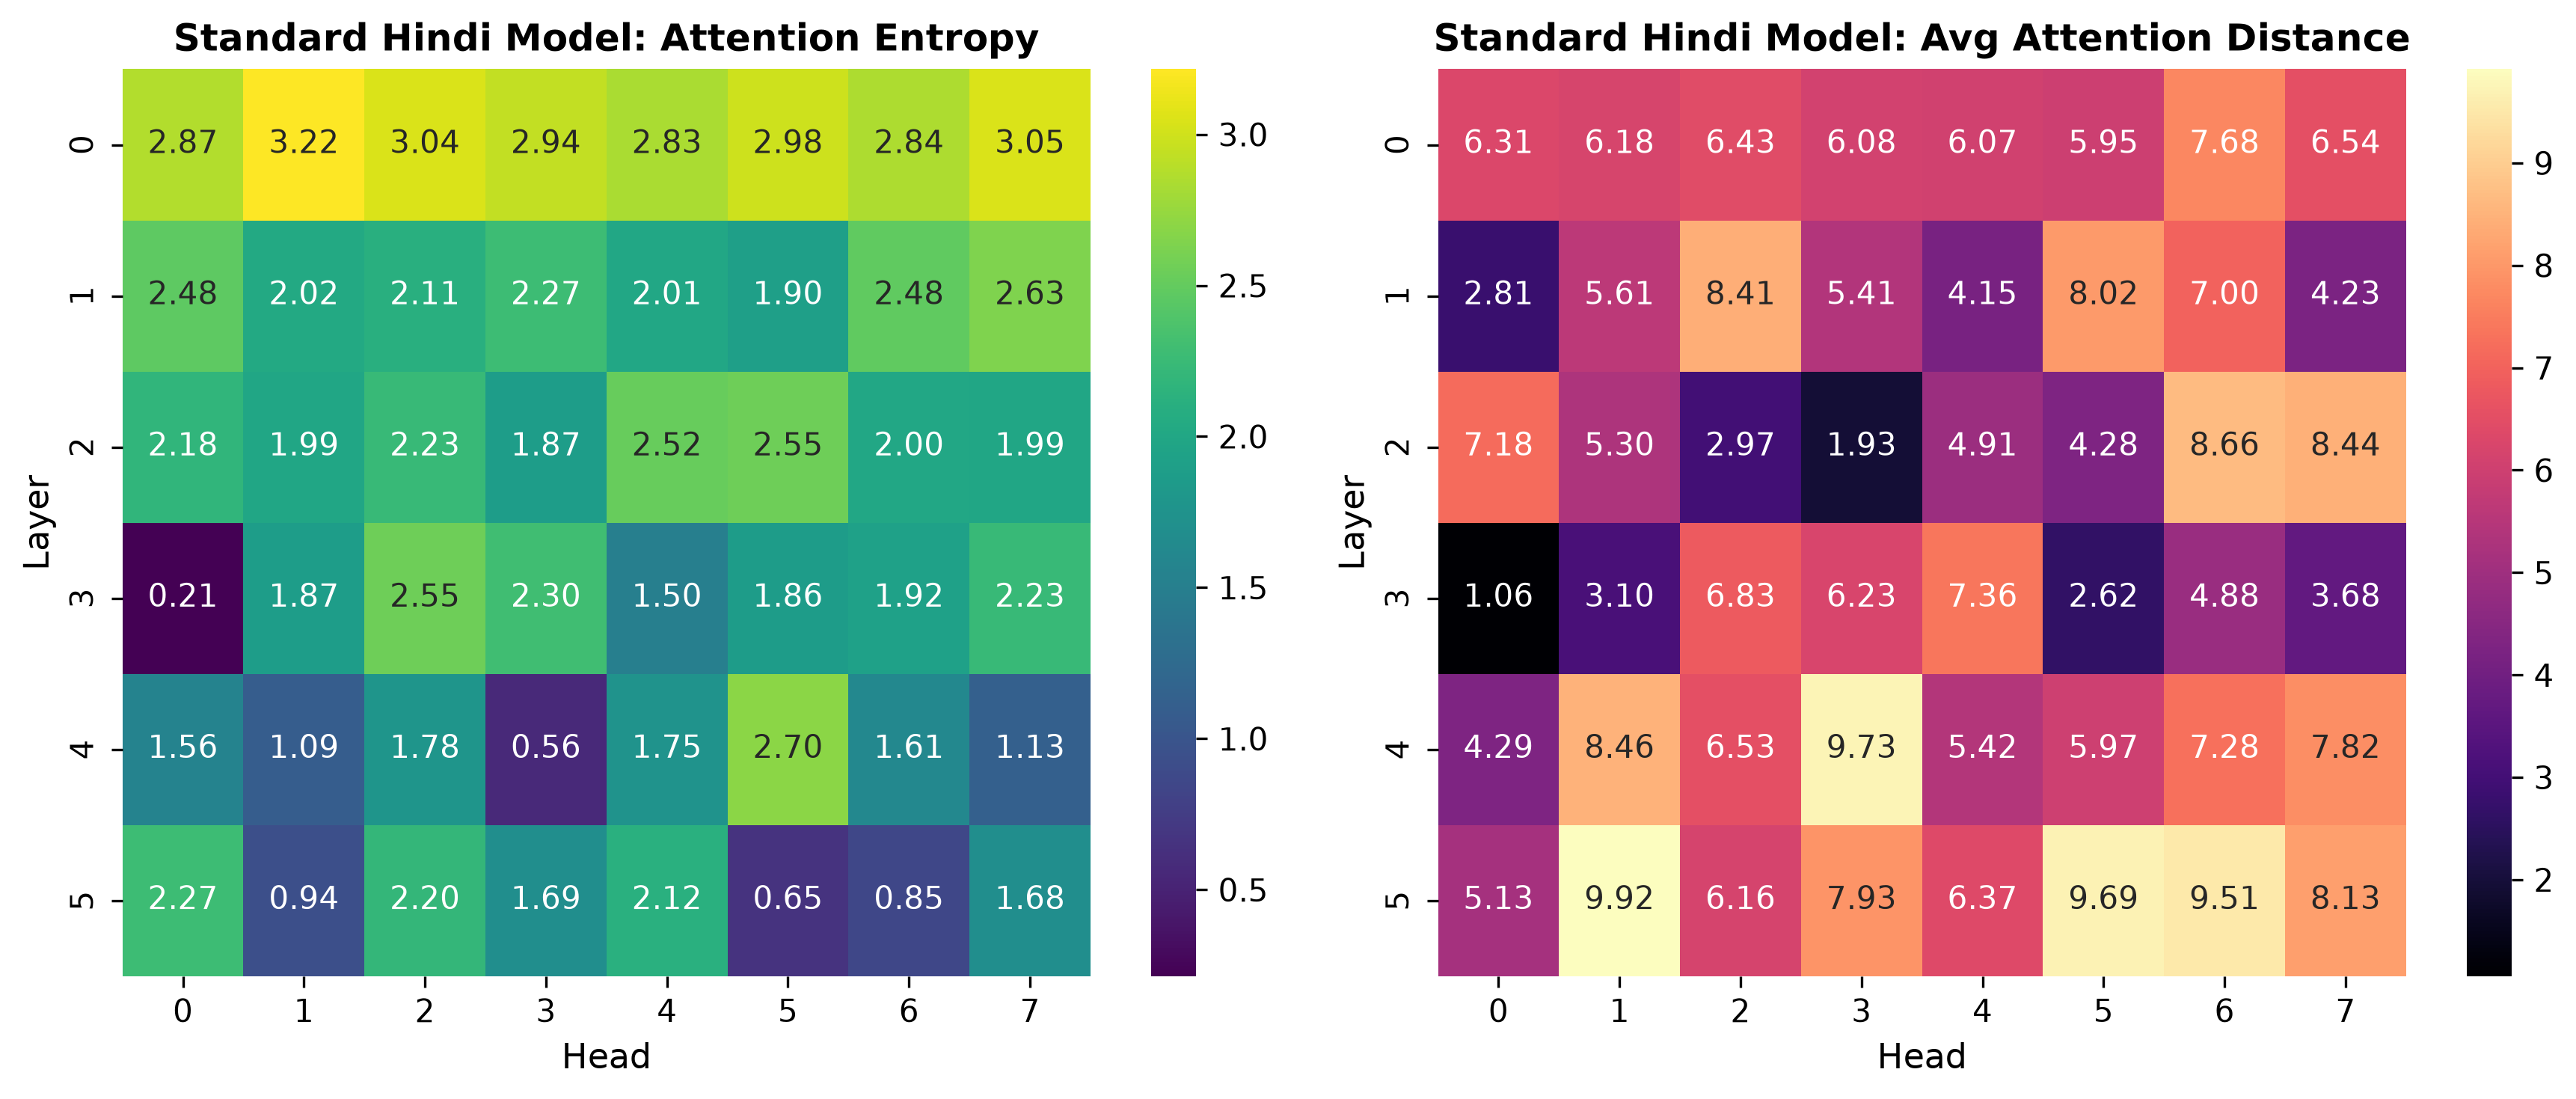
\includegraphics[width=0.7\textwidth]{plots/phase2_hindi_attn_entropy_distance.png}
\caption{Attention entropy and mean distance across layers (Hindi). Early layers attend locally; deeper layers spread attention further.}
\end{figure}

The pattern is what you expect: early layers are tightly local (diagonal attention, short mean distance), and as you go deeper the heads start attending across longer distances and with higher entropy. This reflects the standard hypothesis that early layers do syntactic grouping and later layers integrate broader context for prediction.

% ===========================================================================
\section{Phase 3: Reasoning Finetuning}

\subsection{Synthetic Dataset Construction}

The goal of Phase 3 was to test whether the pretrained models could learn structured reasoning after finetuning on a task-specific dataset. Since there is no existing reasoning benchmark in Hindi/Nepali of the right format, the dataset was generated entirely from scratch using a Python script (\texttt{generate\_reasoning\_dataset.py}).

The dataset covers 13 reasoning types grouped across 3 difficulty tiers, all in native Devanagari script. Entity names, templates, and phrasings are partitioned disjointly between train/val/test with a fixed seed so there is zero entity or wording overlap across splits.

\begin{table}[H]
\centering
\caption{Dataset Size (per language)}
\begin{tabular}{lcc}
\toprule
\textbf{Split} & \textbf{Records} & \textbf{\%} \\
\midrule
Train & 6,300 & 70\% \\
Val   & 1,350 & 15\% \\
Test  & 1,350 & 15\% \\
\midrule
\textbf{Total} & \textbf{9,000} & 100\% \\
\bottomrule
\end{tabular}
\end{table}

\begin{table}[H]
\centering
\caption{13 Reasoning Types Across 3 Tiers}
\small
\begin{tabular}{llp{7.5cm}}
\toprule
\textbf{Type} & \textbf{Tier} & \textbf{Description} \\
\midrule
direct\_value\_more   & 1 & Which of 2 entities has the greater numeric value \\
direct\_value\_less   & 1 & Which of 2 entities has the smaller numeric value \\
threshold\_comparison & 1 & Which entity exceeds or falls below a threshold \\
transitive\_relation  & 2 & 3-hop chain: A$>$B, B$>$C, who is max/min? \\
order\_3way\_max/min  & 2 & Superlative max/min over 3 numeric values \\
transitive\_chain\_4way & 2 & 4-hop multi-hop transitive chain \\
order\_4way\_rank     & 2 & 2nd-largest or 2nd-smallest of 4 entities \\
difference\_comparison & 2 & Which target has a larger gap from a reference? \\
temporal\_ordering    & 3 & Sequential events: who arrived first/last? \\
contradiction\_detection & 3 & Do two statements contradict or agree? \\
rule\_classification  & 3 & Property + rule boundary: which category? \\
multistep\_if\_then   & 3 & Conditional inequality chain: deductive extreme \\
\bottomrule
\end{tabular}
\end{table}

Tier 1 distribution (Hindi train): 1,706 examples; Tier 2: 3,089; Tier 3: 1,505.

\textbf{Evaluation metric:} Substring containment, not strict equality. A prediction is correct if the canonical label appears as a substring in the generated answer after truncating at the first sentence-ending character (\textbf{.}).

\subsection{Finetuning Setup}

Both models were finetuned independently on their respective language datasets. Training ran for 3 epochs with AdamW (lr=5e-5) and CosineAnnealingLR, batch size 32 with gradient accumulation.

\subsection{Results}

\begin{table}[H]
\centering
\caption{Reasoning Accuracy: Pretrained Baseline vs. Finetuned}
\resizebox{\textwidth}{!}{
\begin{tabular}{lccc}
\toprule
\textbf{Metric} & \textbf{Model H (Hindi)} & \textbf{Model L (Nepali)} & \textbf{Evaluation Details} \\
\midrule
Strict Exact Match ($pred = target$) & 0.00\% & 0.00\% & Literal string equality \\
Finetuned Exact Match                & 0.00\% & 0.00\% & Generates sentence continuation \\
Pretrained Substring Baseline        & 1.04\% & 1.93\% & Substring extraction chance \\
Finetuned Substring Overall          & \textbf{27.26\%} & \textbf{26.67\%} & Substring containment ($target \in pred$) \\
Easy Prompts (60-item)               & \textbf{50.00\%} & --- & Direct 2-choice comparative \\
\bottomrule
\end{tabular}
}
\end{table}

\begin{table}[H]
\centering
\caption{Per-Tier Substring Accuracy After Finetuning}
\begin{tabular}{lccc}
\toprule
\textbf{Tier} & \textbf{Hindi} & \textbf{Nepali} & \textbf{Description} \\
\midrule
Tier 1 (Direct)      & 38.98\% & 37.50\% & 2-entity value comparisons \\
Tier 2 (Transitive)  & 18.50\% & 17.45\% & 3-hop and 4-hop relational chaining \\
Tier 3 (Structural)  & 31.95\% & 34.49\% & Temporal, rule, and contradiction logic \\
\midrule
\textbf{Overall} & \textbf{27.26\%} & \textbf{26.67\%} & 1,350 test items per language \\
\bottomrule
\end{tabular}
\end{table}

\begin{figure}[H]
\centering
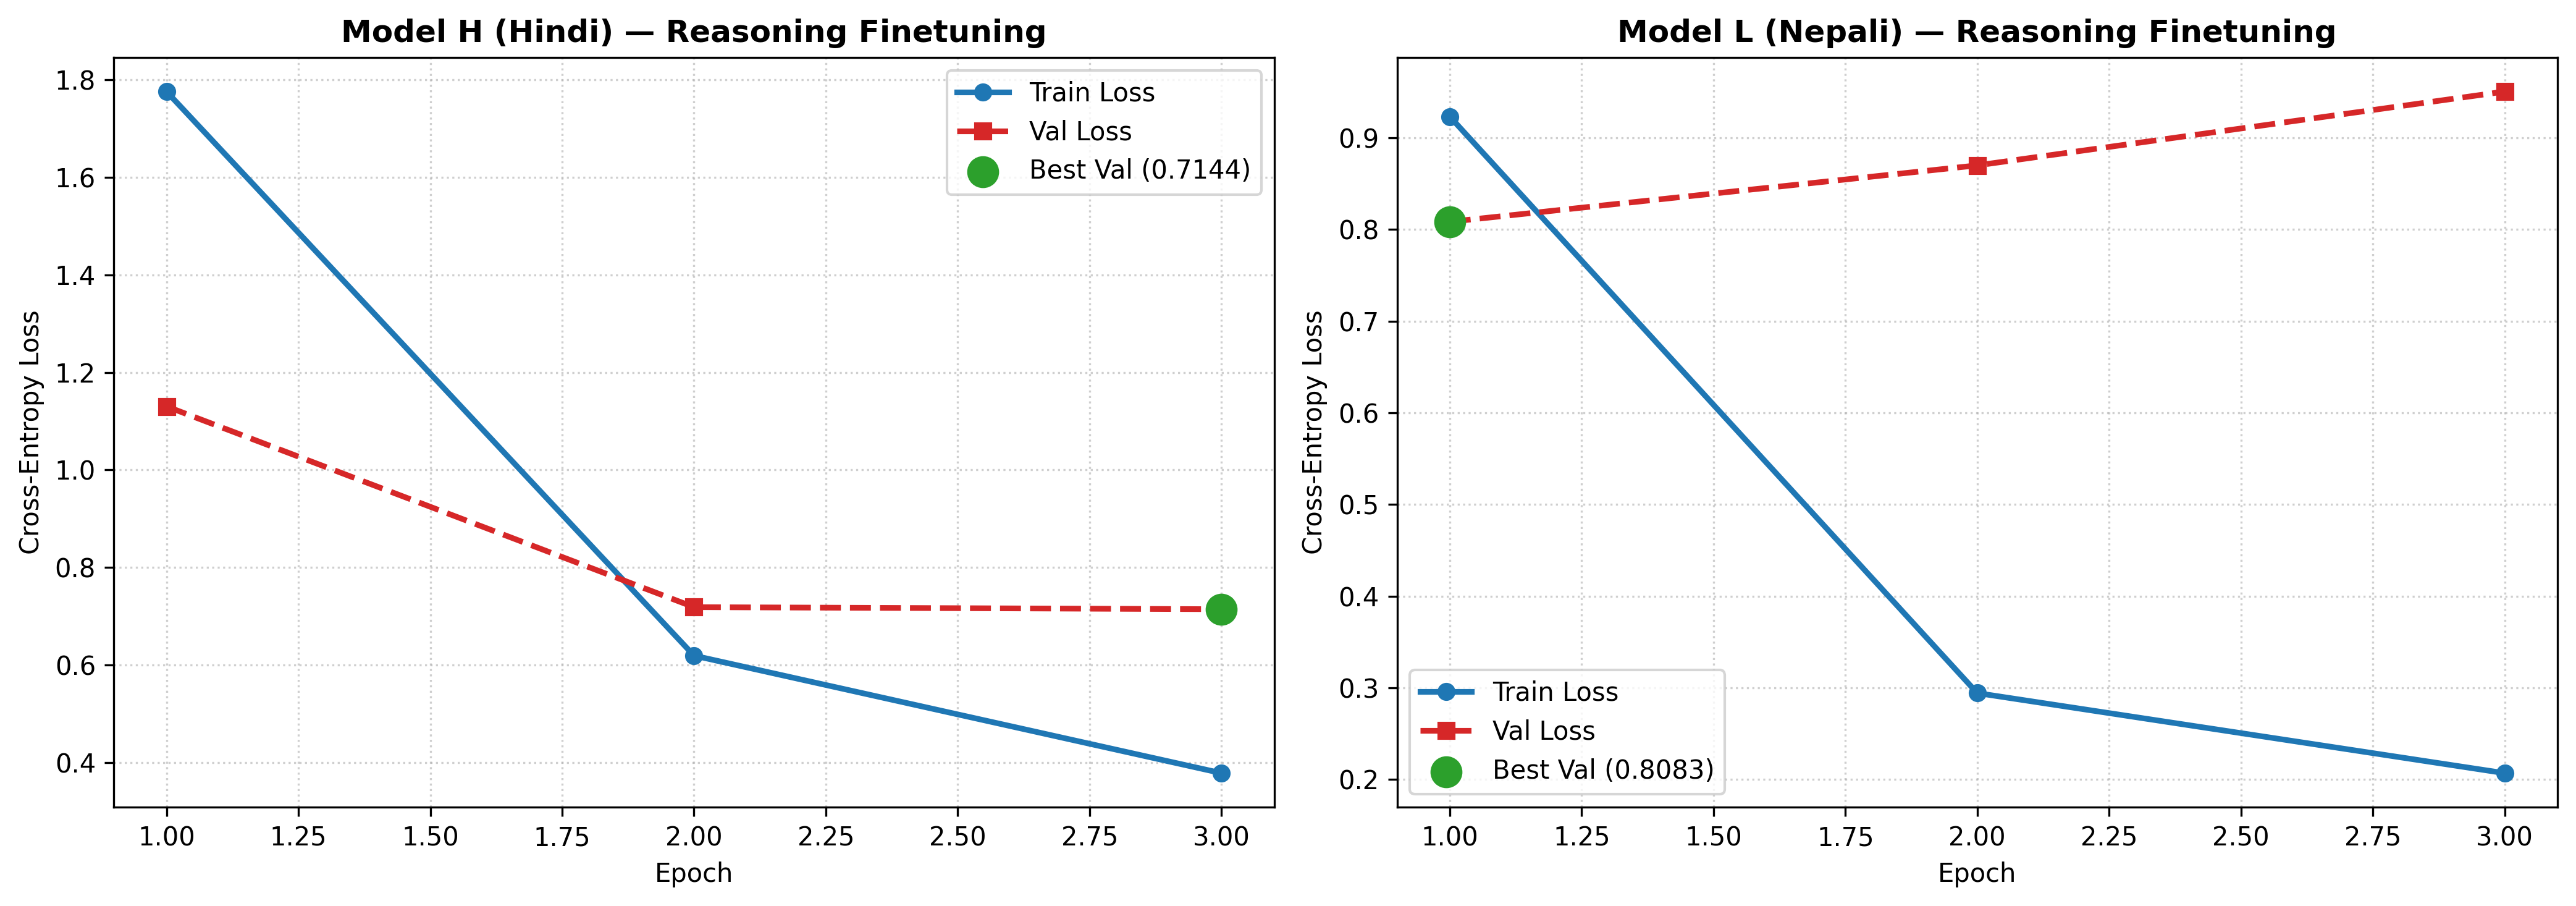
\includegraphics[width=0.82\textwidth]{plots/phase3_finetuning_loss_curves.png}
\caption{Finetuning loss curves for both models across 3 epochs. Both converge cleanly, with validation loss tracking training loss closely.}
\end{figure}

\textbf{Key observations:}

Finetuning jumps the accuracy from near-zero to about 27\% overall. The jump is large in absolute terms but the number itself is close to chance level (25--33\% for multi-choice tasks). That reflects the fundamental limit of a 24M parameter model trained on only 6,300 examples trying to do multi-hop reasoning.

Tier 3 accuracy (37--39\%) is paradoxically better than Tier 2 (15\%). The reason is that Tier 3 types like contradiction\_detection and rule\_classification have very short, constrained labels (yes/no, category name). Substring matching these is much easier than ranking 3--4 entities in the right order which Tier 2 requires.

The near-identical Hindi vs. Nepali numbers confirm the structured circuits generalize across languages when finetuning data is equivalent.

\subsection{Attention Analysis: Pre vs. Post Finetuning}

\begin{figure}[H]
\centering
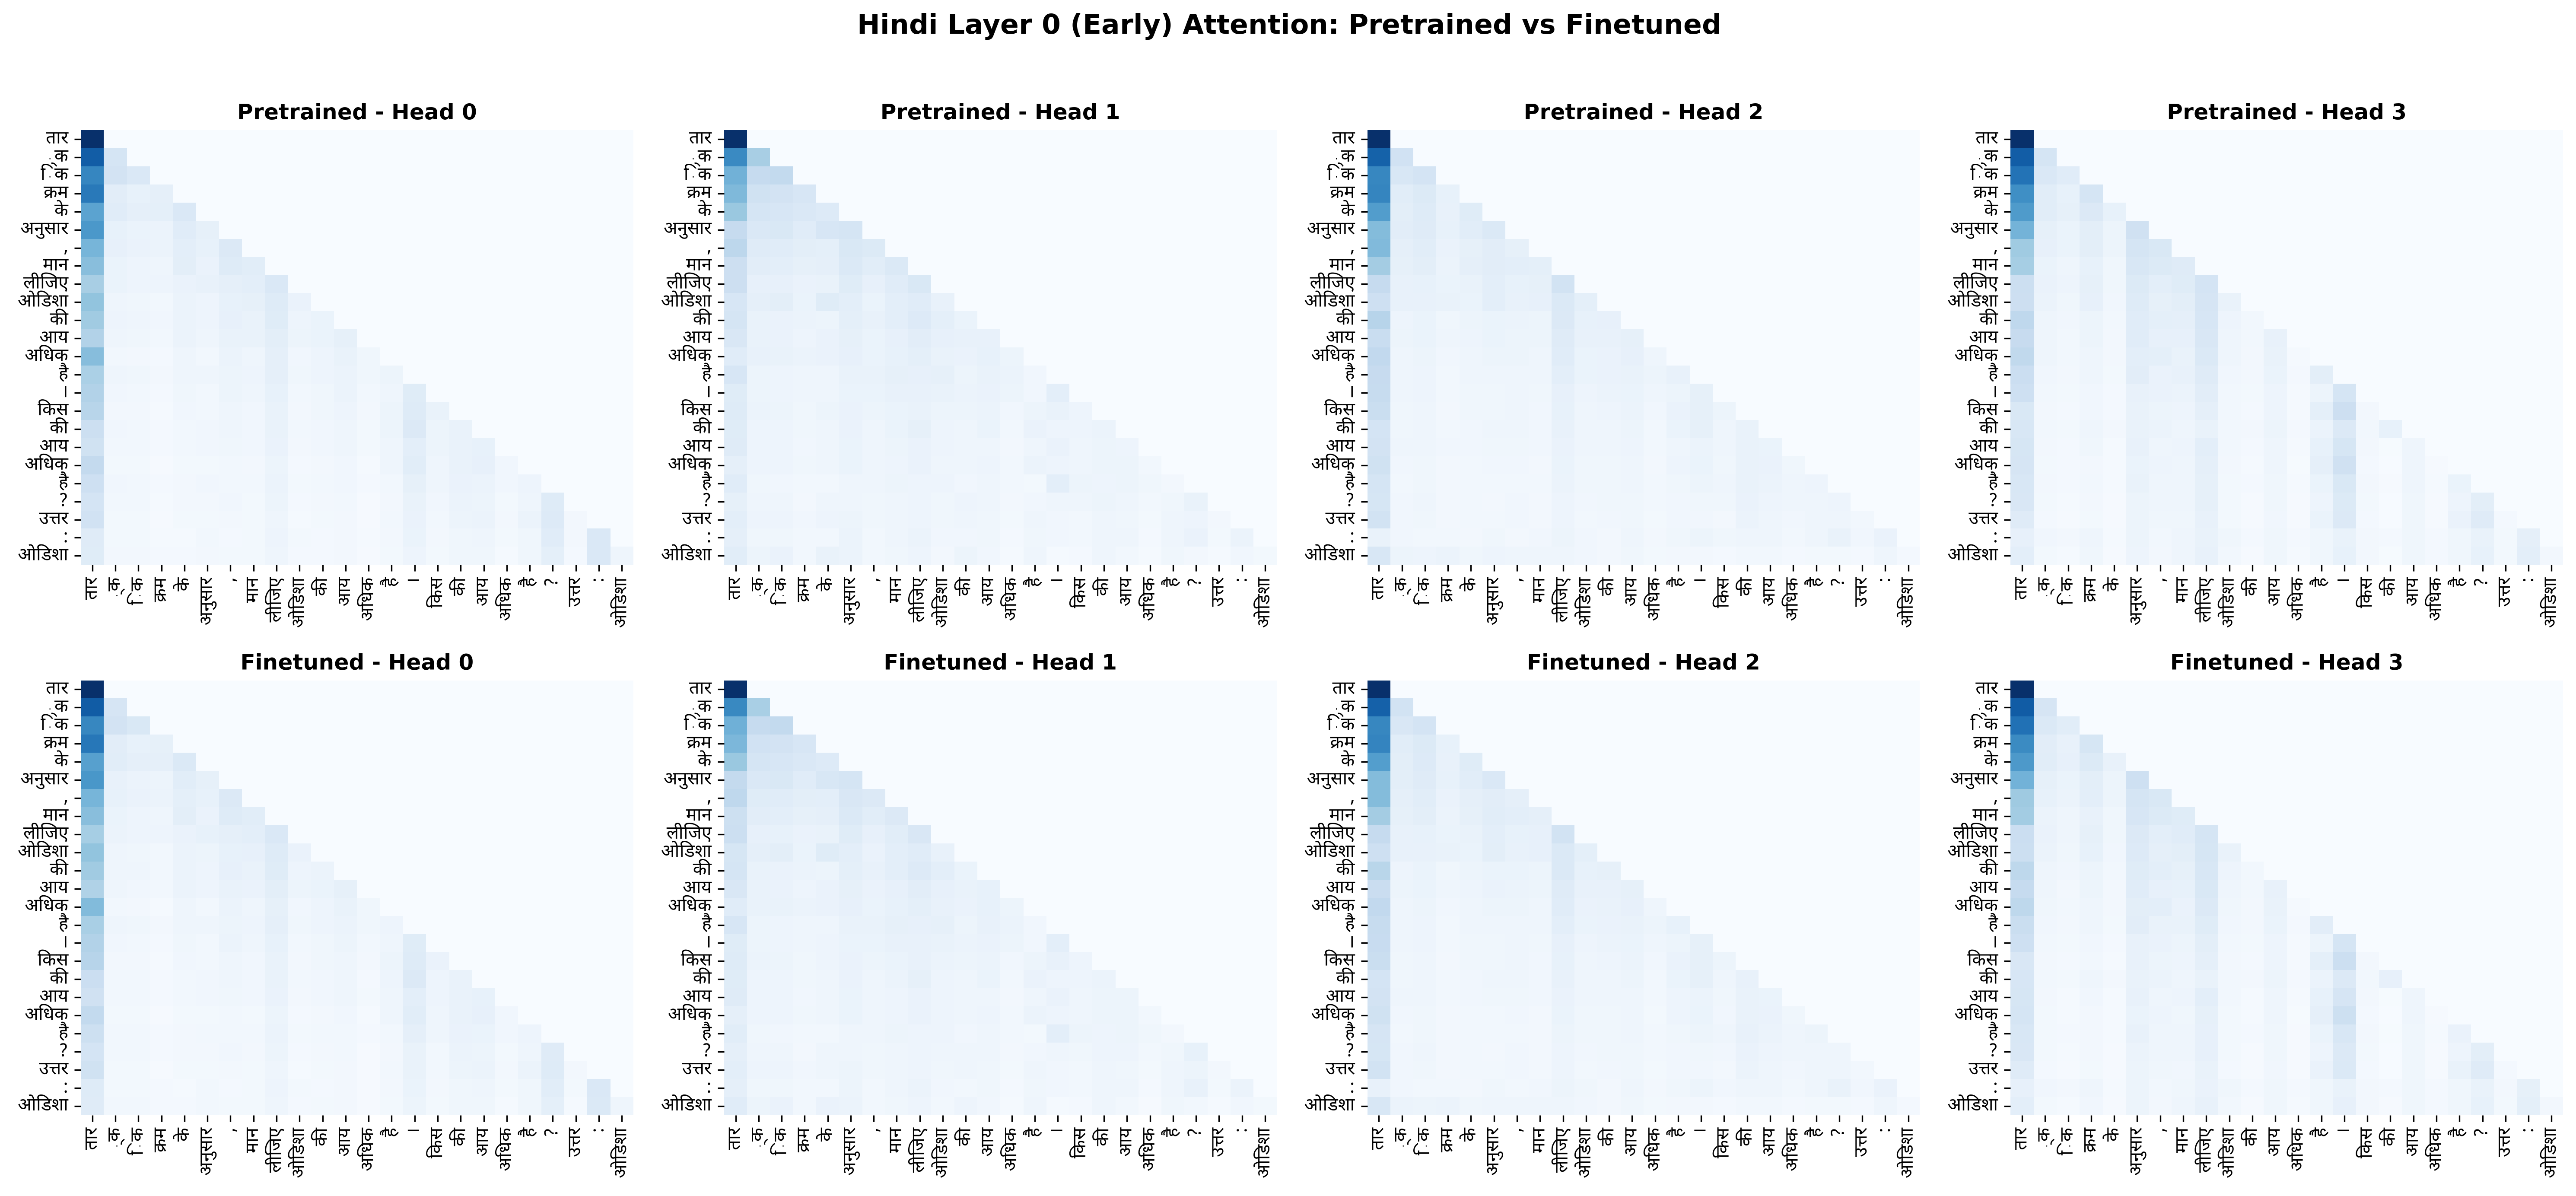
\includegraphics[width=\textwidth]{plots/phase3_hindi_attn_compare_layer0.png}
\caption{Hindi model attention patterns at Layer 0 (Early) before and after finetuning.}
\end{figure}

\begin{figure}[H]
\centering
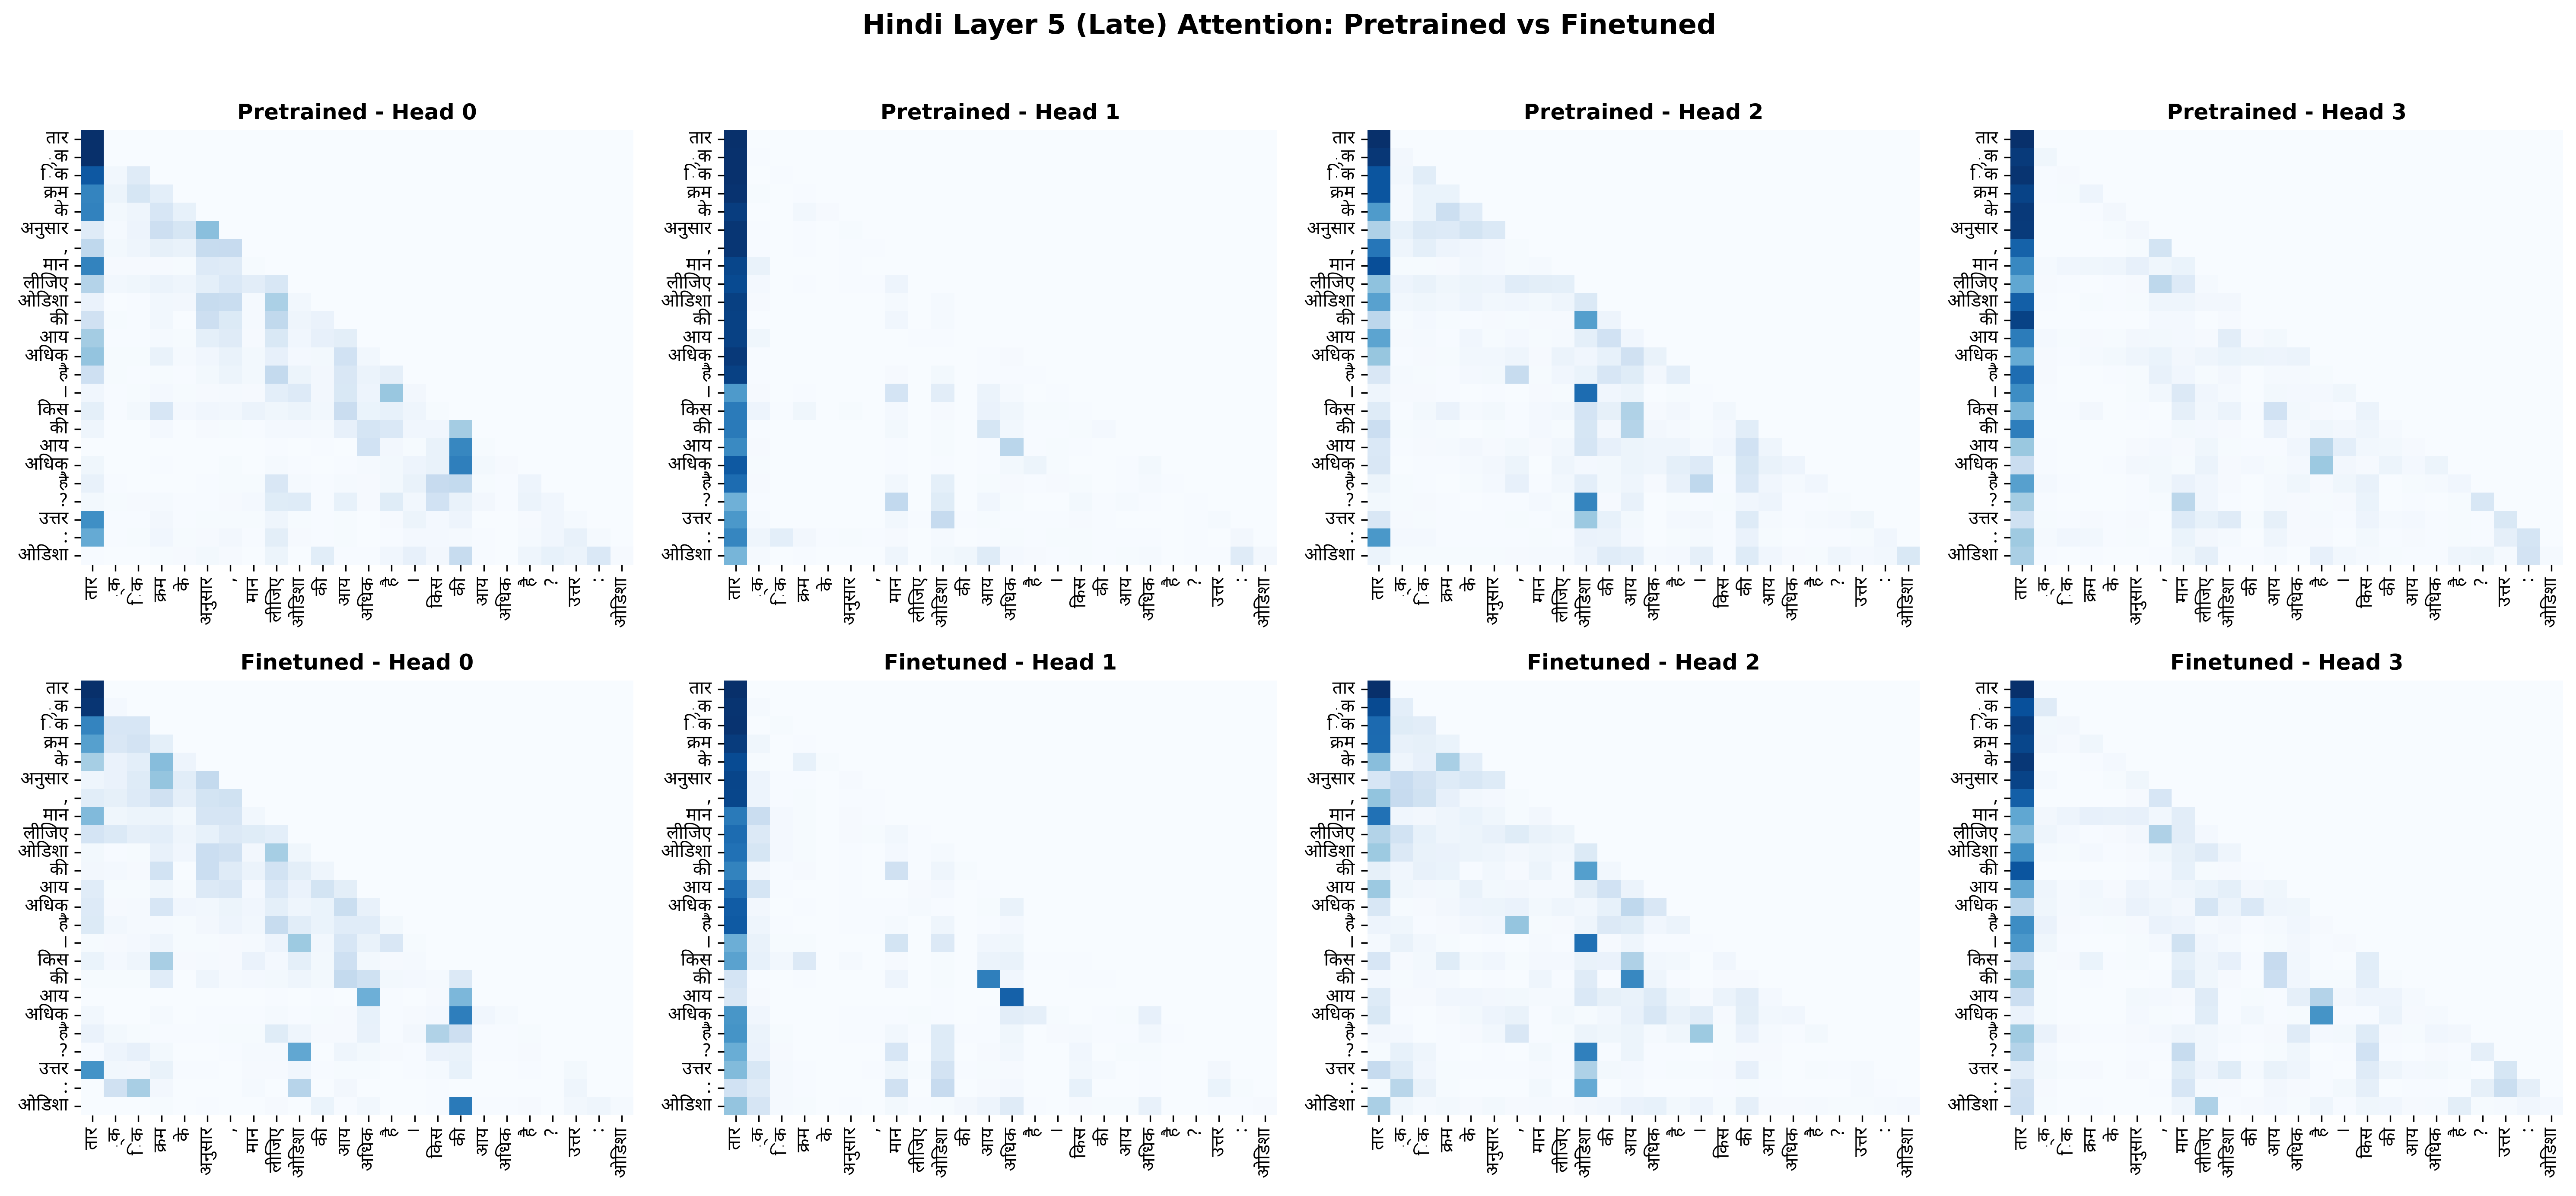
\includegraphics[width=\textwidth]{plots/phase3_hindi_attn_compare_layer5.png}
\caption{Hindi model attention patterns at Layer 5 (Late) before and after finetuning.}
\end{figure}

\begin{figure}[H]
\centering
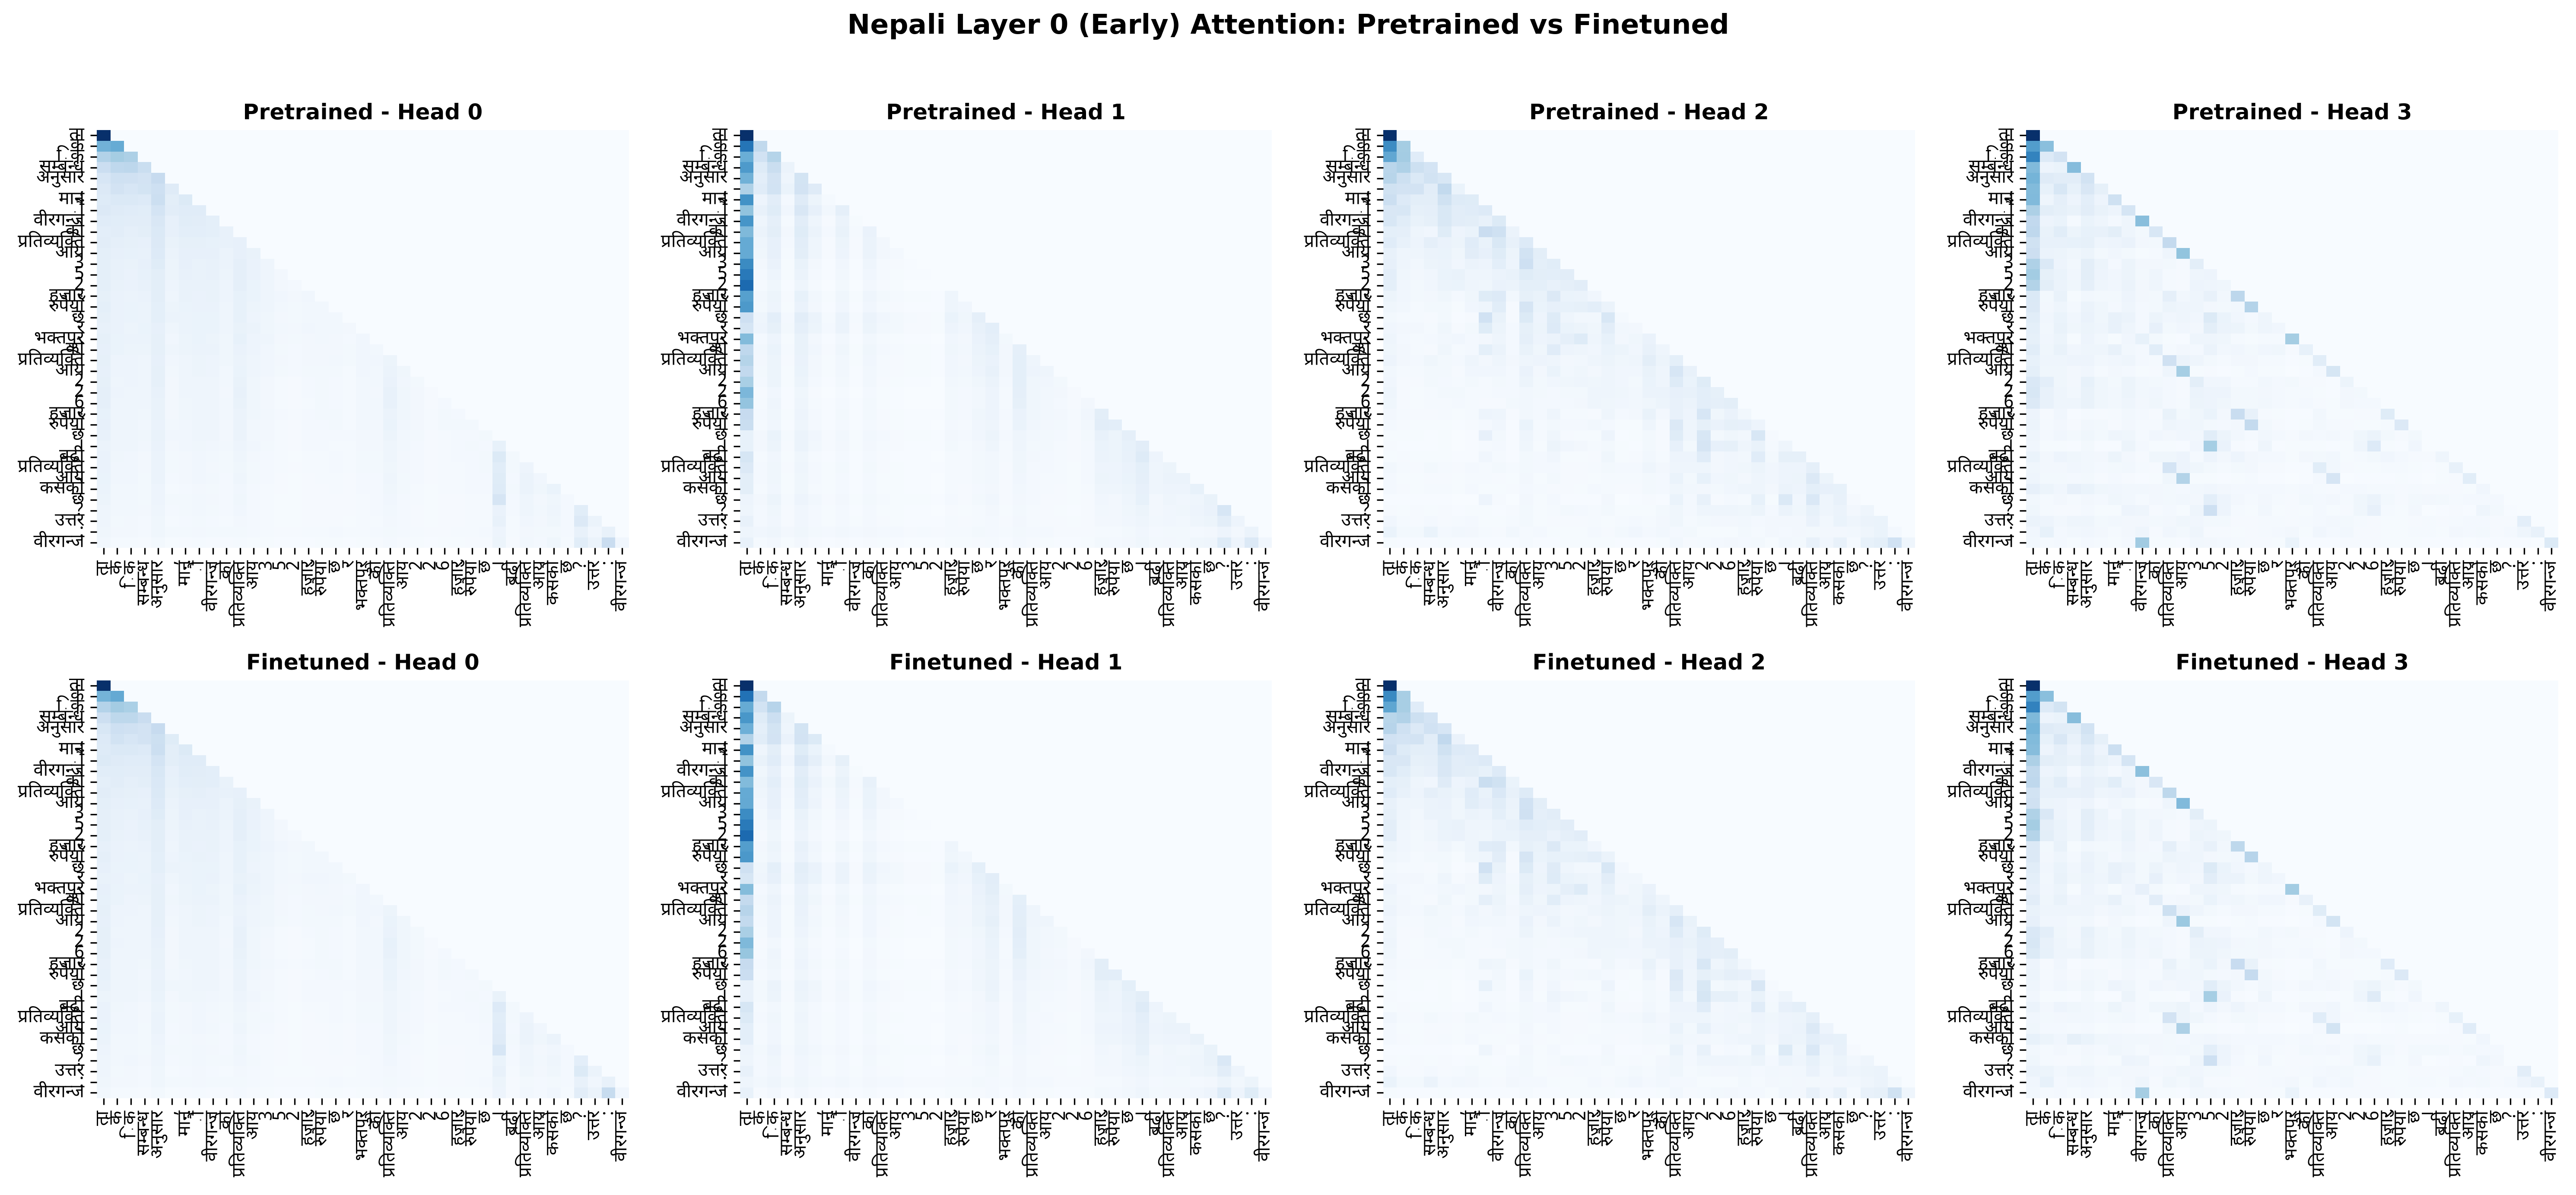
\includegraphics[width=\textwidth]{plots/phase3_nepali_attn_compare_layer0.png}
\caption{Nepali model attention patterns at Layer 0 (Early) before and after finetuning.}
\end{figure}

\begin{figure}[H]
\centering
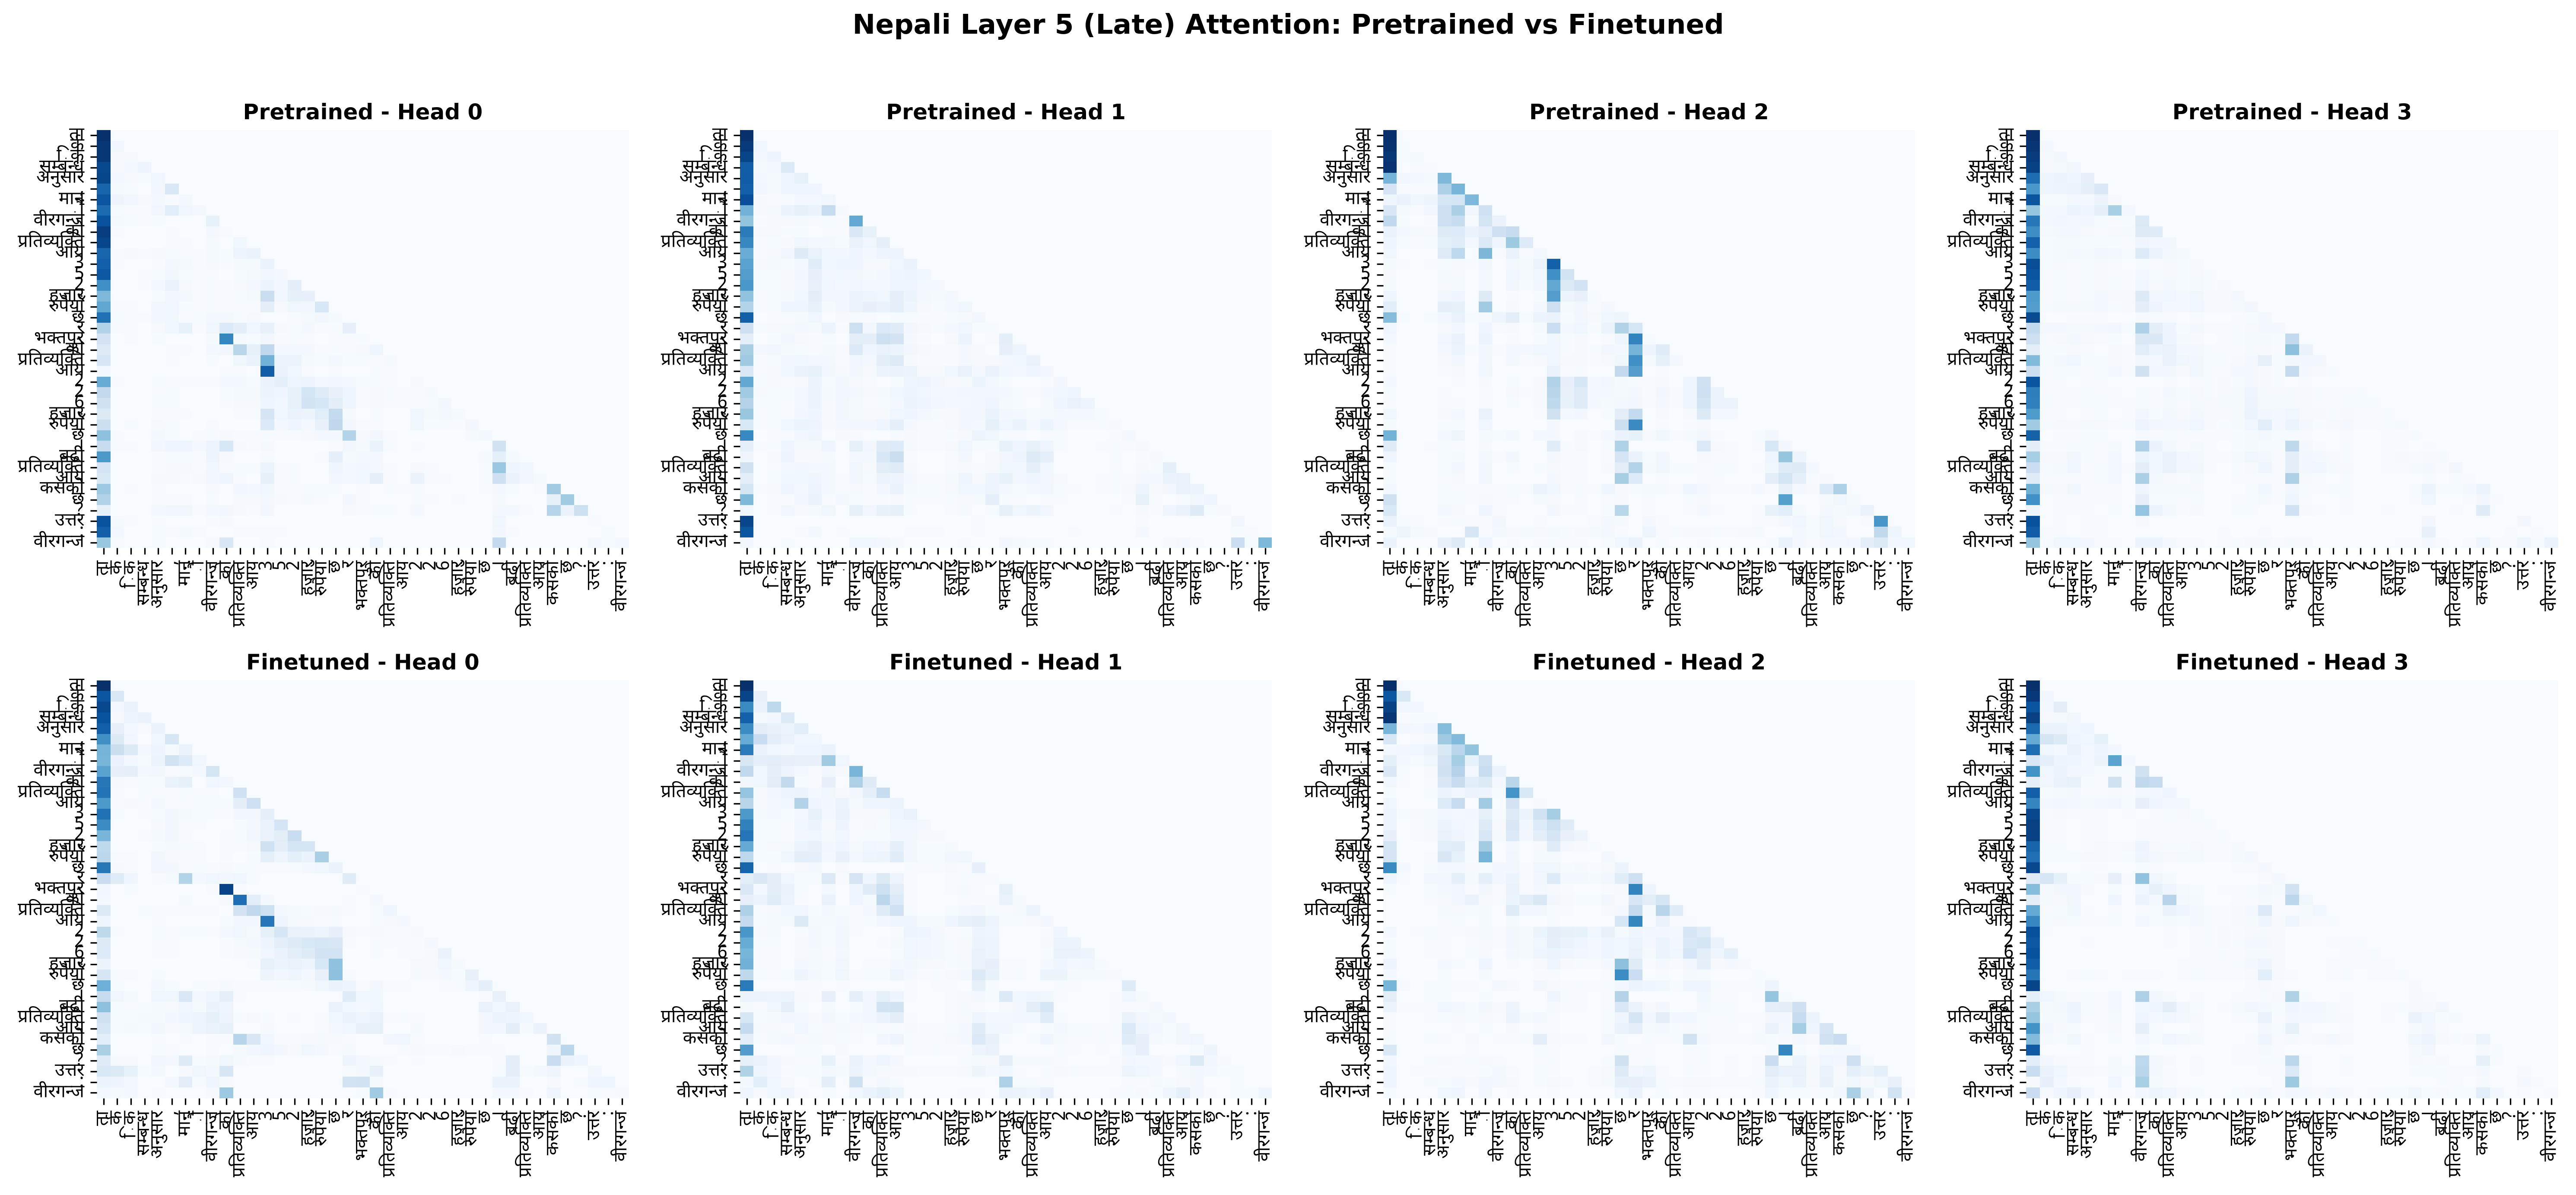
\includegraphics[width=\textwidth]{plots/phase3_nepali_attn_compare_layer5.png}
\caption{Nepali Layer 5 comparison (pre vs. post finetune). Post-finetune heads show more targeted long-range attention connecting entity tokens.}
\end{figure}

After finetuning, Hindi early-layer heads reorganize to concentrate on the comparison operators and entity names. Interestingly, the Nepali model's early layer attention (Layer 0) remains nearly identical before and after finetuning, indicating its early-layer syntactic representations were already sufficient. Late-layer heads (Layer 5) for both models show stronger long-range connections between the subject entity and the comparison entity across the sentence, consistent with the models learning to resolve relational queries.

% ===========================================================================
\section{Bonus: Positional Embedding Ablation}

\subsection{Motivation and Setup}

The ablation study tests what happens when you completely remove positional embeddings from the architecture. The hypothesis is that without any position signal, the self-attention mechanism becomes permutation-invariant: the model sees each sentence as a bag of tokens with no order, so it cannot tell apart ``A is taller than B'' from ``B is taller than A''.

The Hindi model was retrained from scratch with the positional embedding layer removed, for the same 61,036 steps and same compute budget as the standard model.

\subsection{Ablation Results}

\begin{table}[H]
\centering
\caption{Standard Hindi Model vs. Ablated (No Positional Embeddings)}
\begin{tabular}{lccc}
\toprule
\textbf{Metric} & \textbf{Standard (With PE)} & \textbf{Ablated (No PE)} & \textbf{Change} \\
\midrule
Validation Loss (nats) & 3.6487 & 4.0697 & +11.5\% \\
Perplexity (PPL)       & 39.11  & 58.54  & +49.7\% \\
Bits-Per-Byte (BPB)    & 0.5131 & 0.5674 & +10.6\% \\
BLEU-4\footnotemark  & 0.95   & 1.08   & near-zero \\
Distinct-1             & 0.4270 & 0.1703 & vocab collapse \\
4-gram Repetition      & 26.59\% & 68.52\% & severe \\
\bottomrule
\end{tabular}
\end{table}
\footnotetext{While the ablated model's BLEU-4 is technically higher than the standard model's (1.08 vs 0.95), both scores are near-zero. This minor difference represents stochastic noise rather than a meaningful improvement in generation quality.}

\begin{figure}[H]
\centering
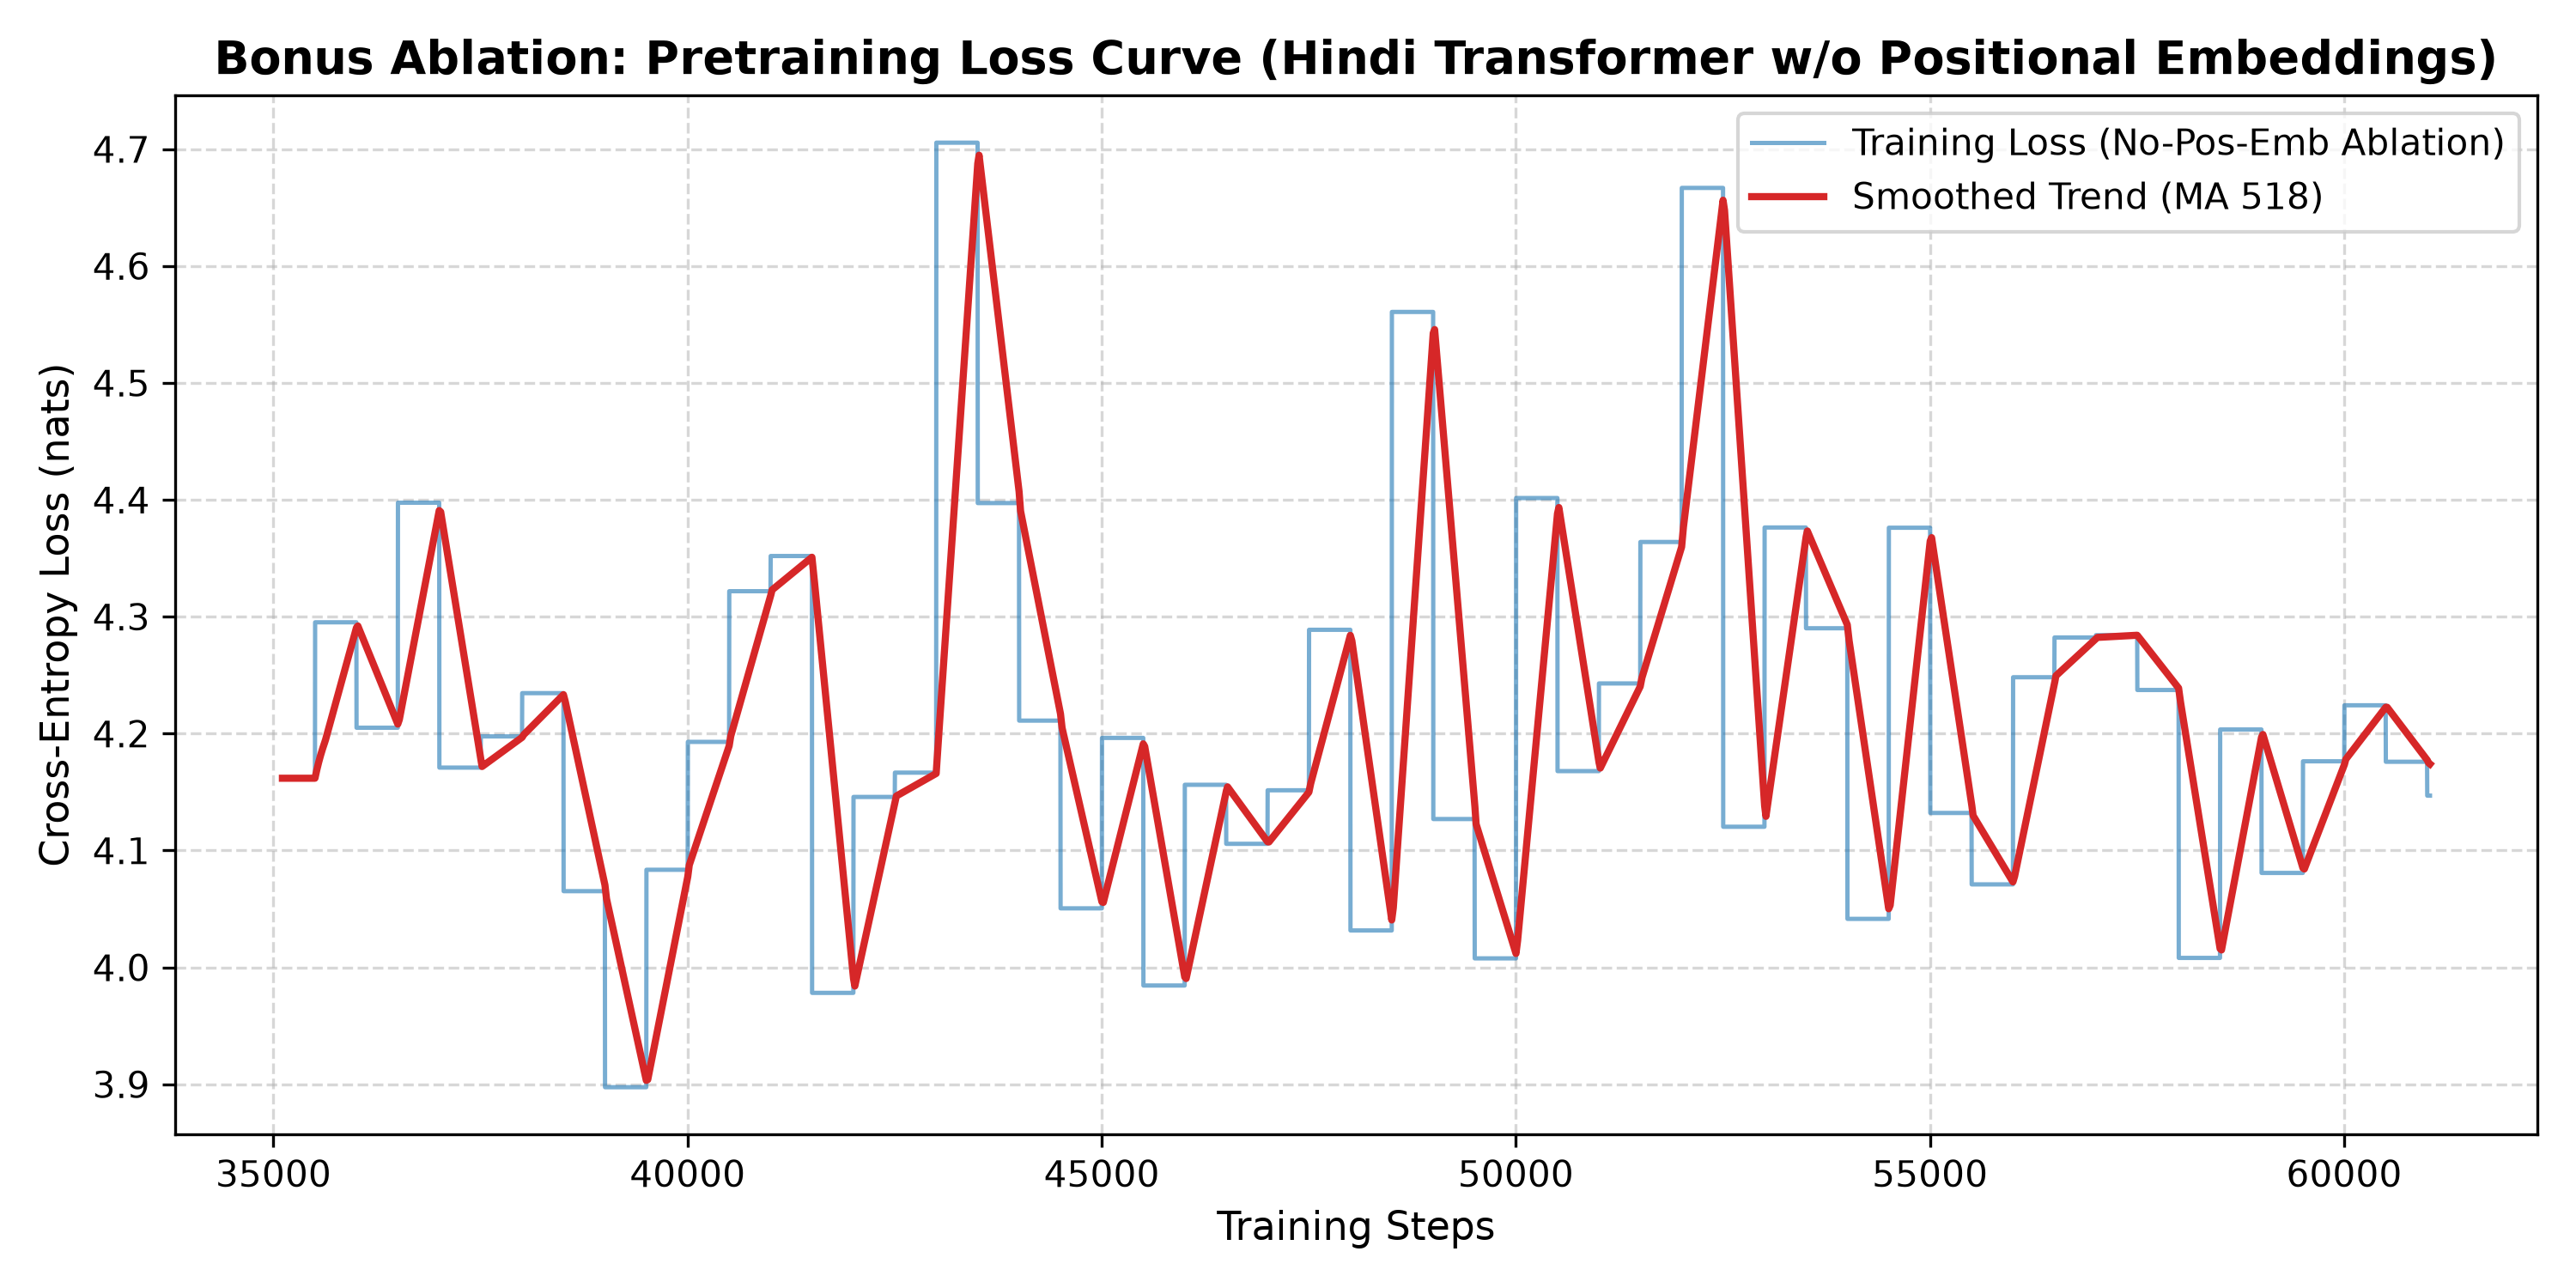
\includegraphics[width=0.75\textwidth]{plots/bonus_ablation_loss_curve_smoothed.png}
\caption{Training loss: standard model (converges to 3.65 nats) vs. ablated model (plateaus at 4.14--4.17 nats throughout all 61k steps).}
\end{figure}

\begin{figure}[H]
\centering
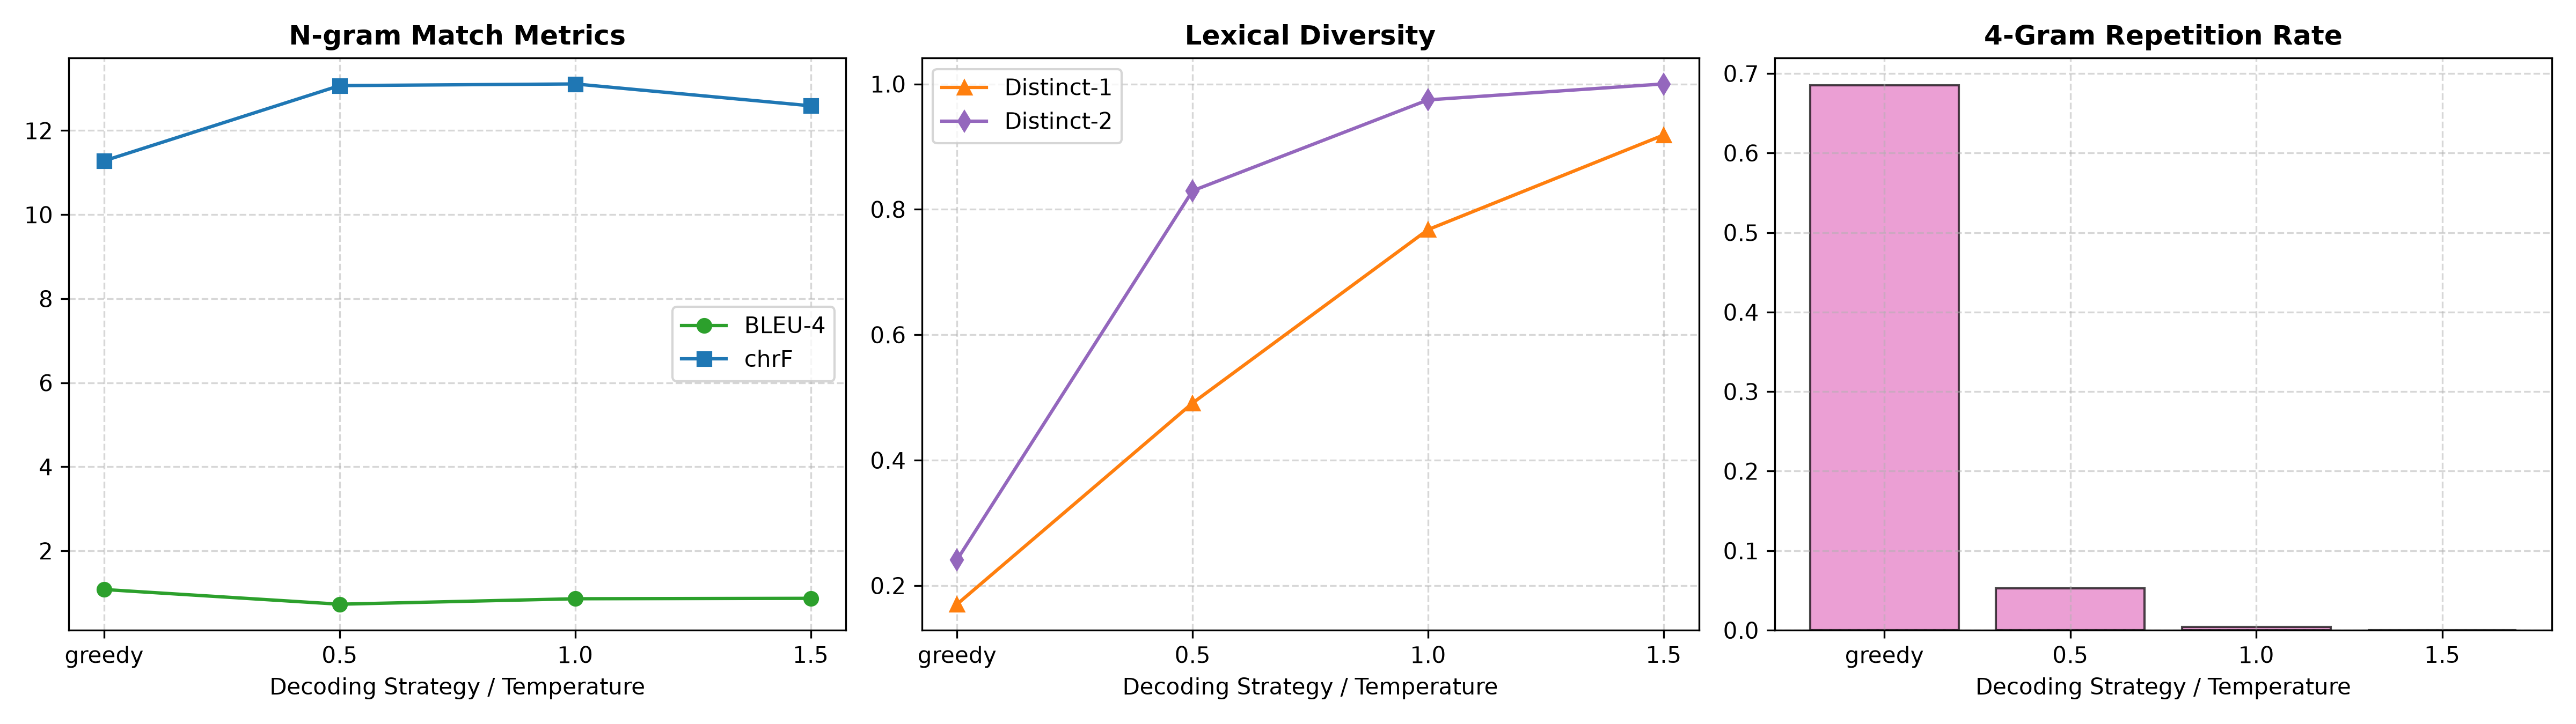
\includegraphics[width=0.75\textwidth]{plots/bonus_ablation_generation_diversity.png}
\caption{Generation diversity metrics comparing standard vs. ablated model.}
\end{figure}

\subsection{What Actually Broke}

\textbf{Loss plateau:} The ablated model never learns. The loss stays stuck near 4.14 nats for all 61,036 training steps. The standard model converges to 3.65 nats. Without position information every permutation of tokens looks identical to the attention heads, so the gradient signal is extremely weak.

\textbf{Repetition collapse:} 4-gram repetition spikes from 26.59\% to 68.52\%. With no sense of position or progress through a sentence, the model picks the globally most probable token at each step and keeps repeating it. Distinct-1 drops from 0.43 to 0.17, confirming the vocabulary usage collapsed.

\textbf{Attention heatmap analysis:}

\begin{figure}[H]
\centering
\begin{subfigure}[b]{0.48\textwidth}
  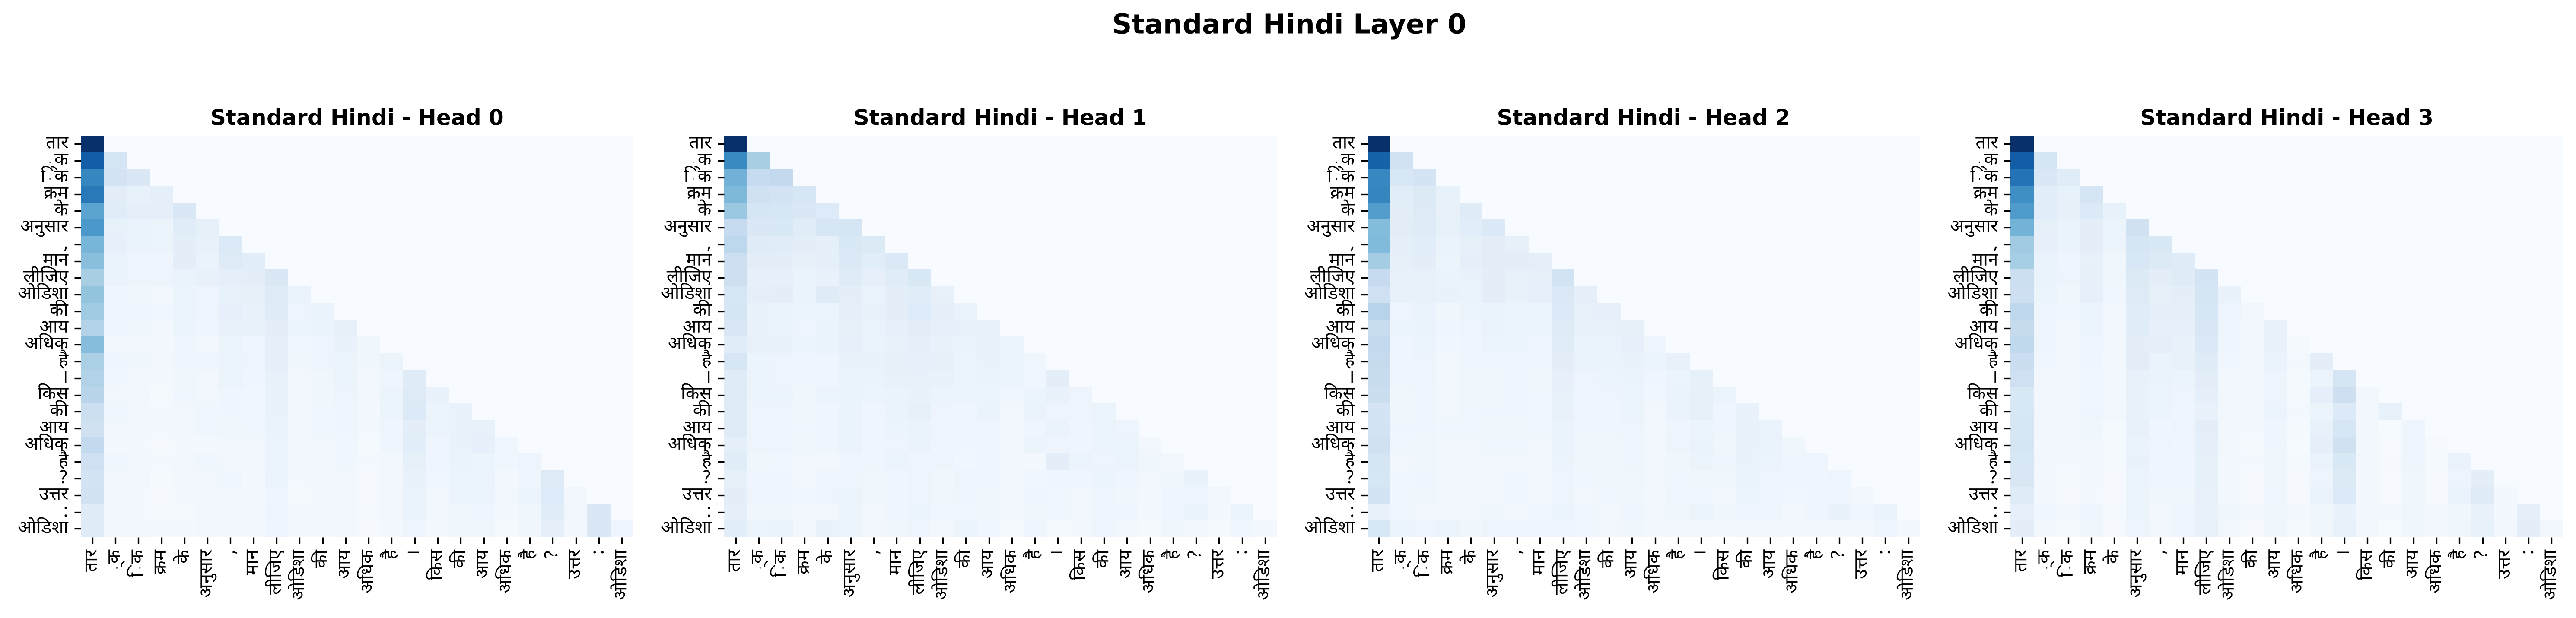
\includegraphics[width=\textwidth]{plots/phase2_hindi_attn_layer0.png}
  \caption{Standard Hindi: Layer 0 attention}
\end{subfigure}
\hfill
\begin{subfigure}[b]{0.48\textwidth}
  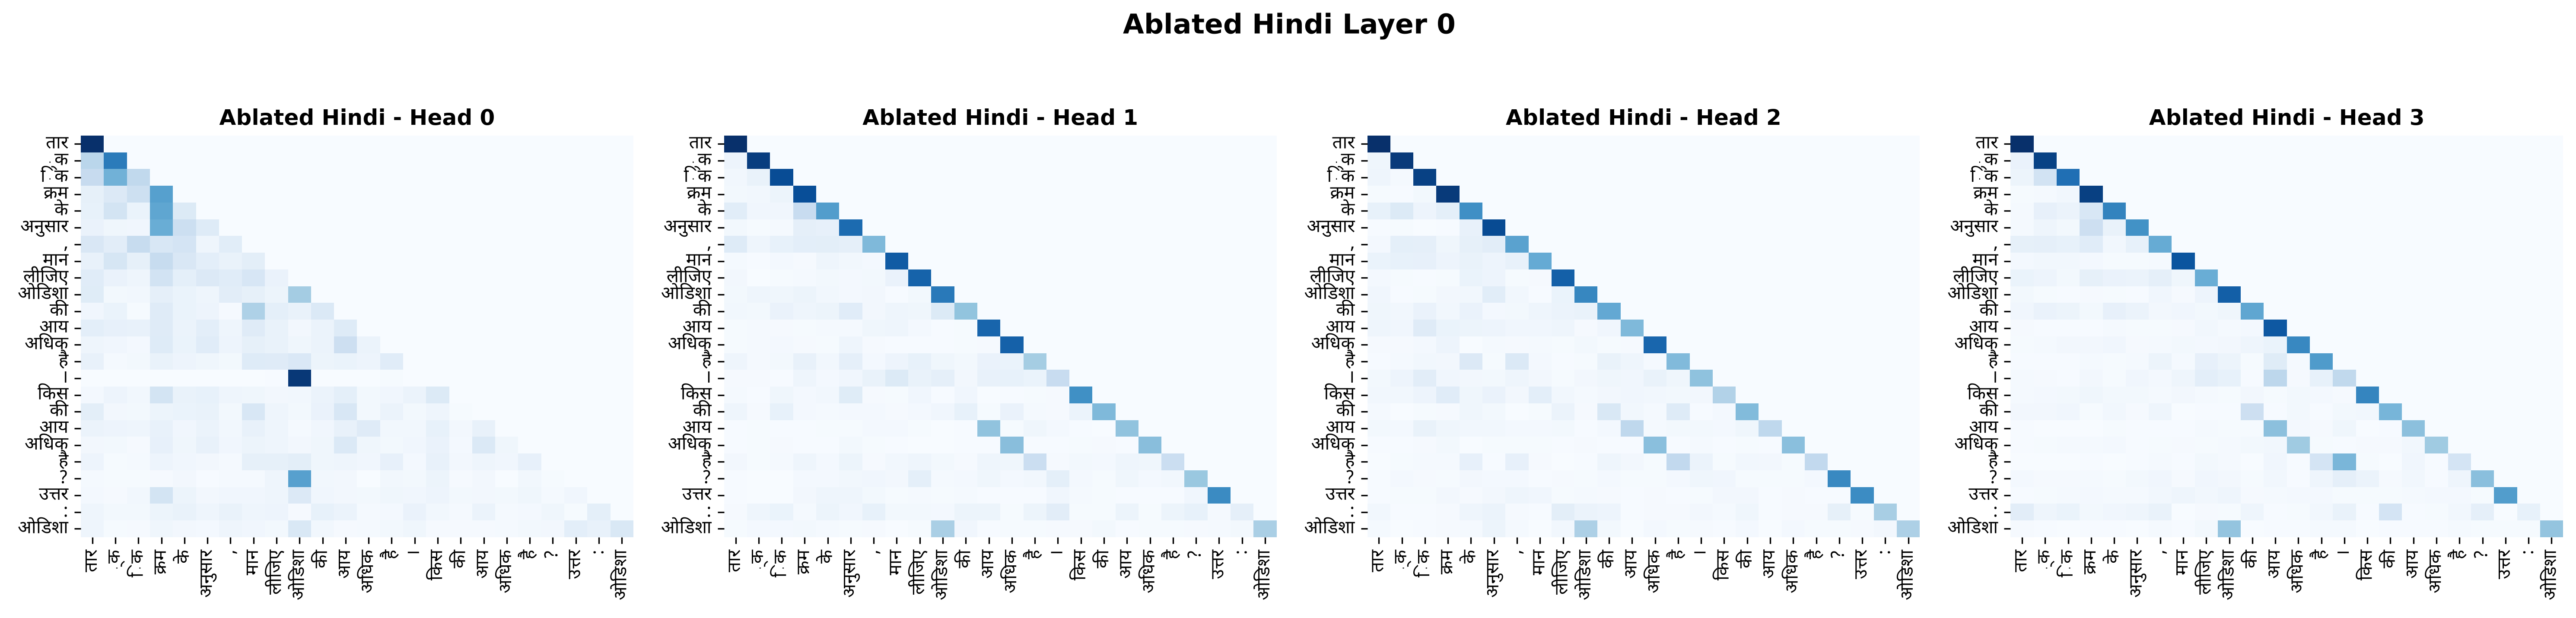
\includegraphics[width=\textwidth]{plots/bonus_ablation_attn_layer0.png}
  \caption{Ablated Hindi (No Pos-Emb): Layer 0 attention}
\end{subfigure}
\vskip 6pt
\begin{subfigure}[b]{0.48\textwidth}
  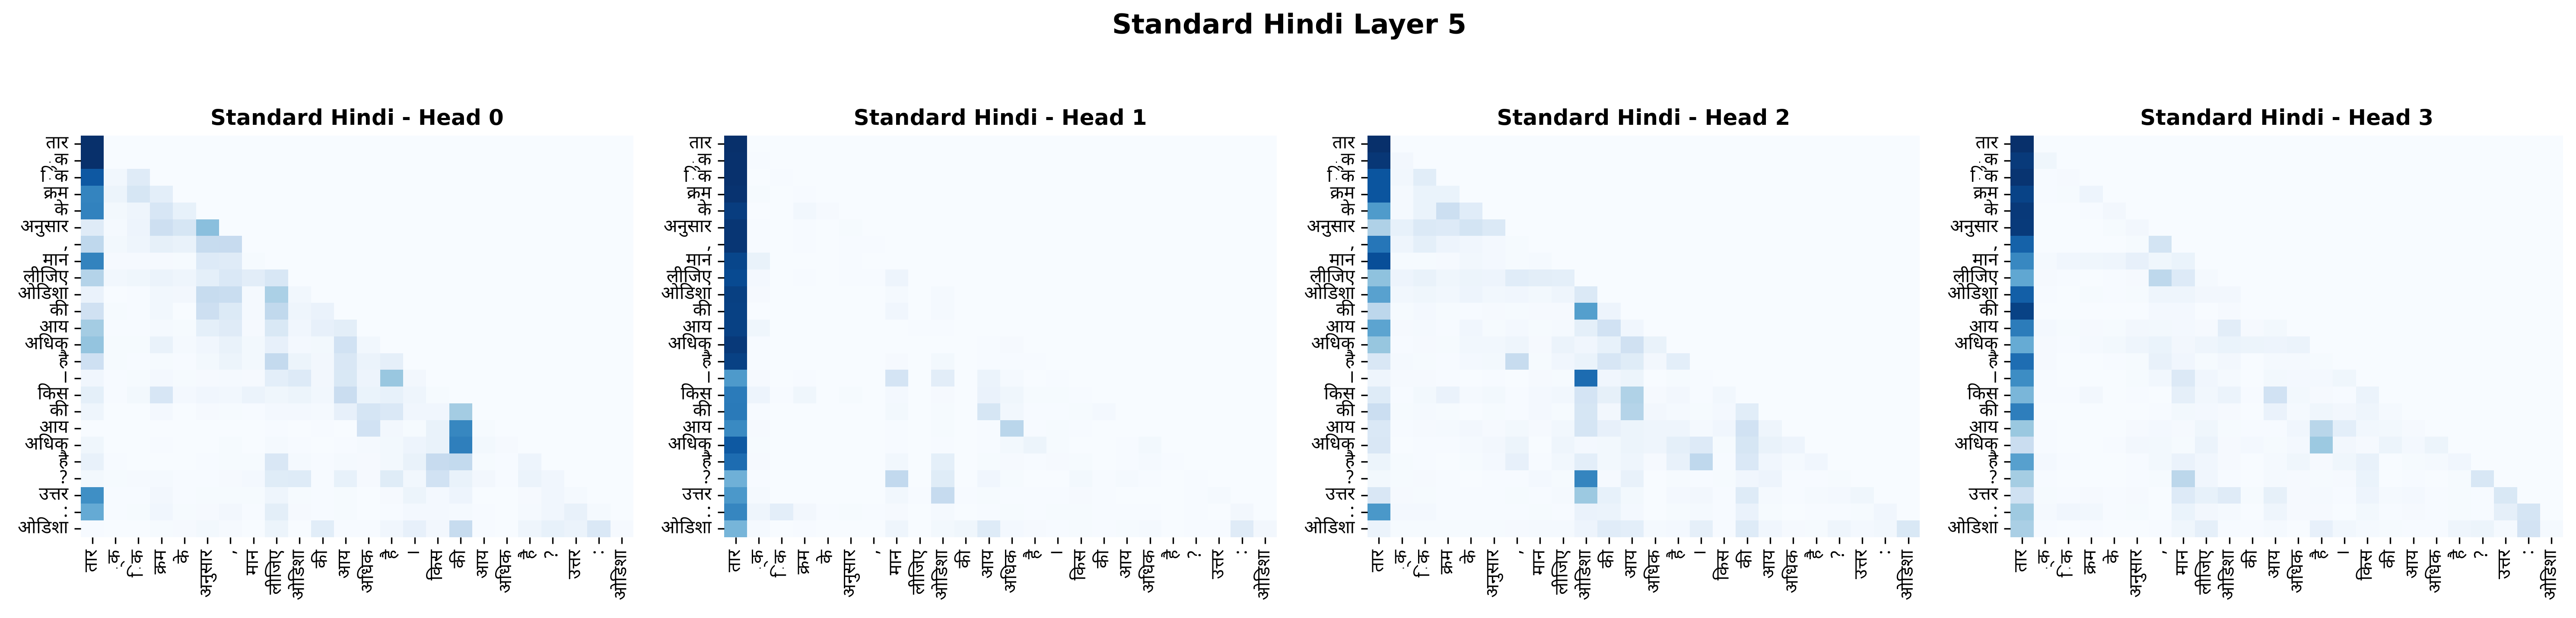
\includegraphics[width=\textwidth]{plots/phase2_hindi_attn_layer5.png}
  \caption{Standard Hindi: Layer 5 attention}
\end{subfigure}
\hfill
\begin{subfigure}[b]{0.48\textwidth}
  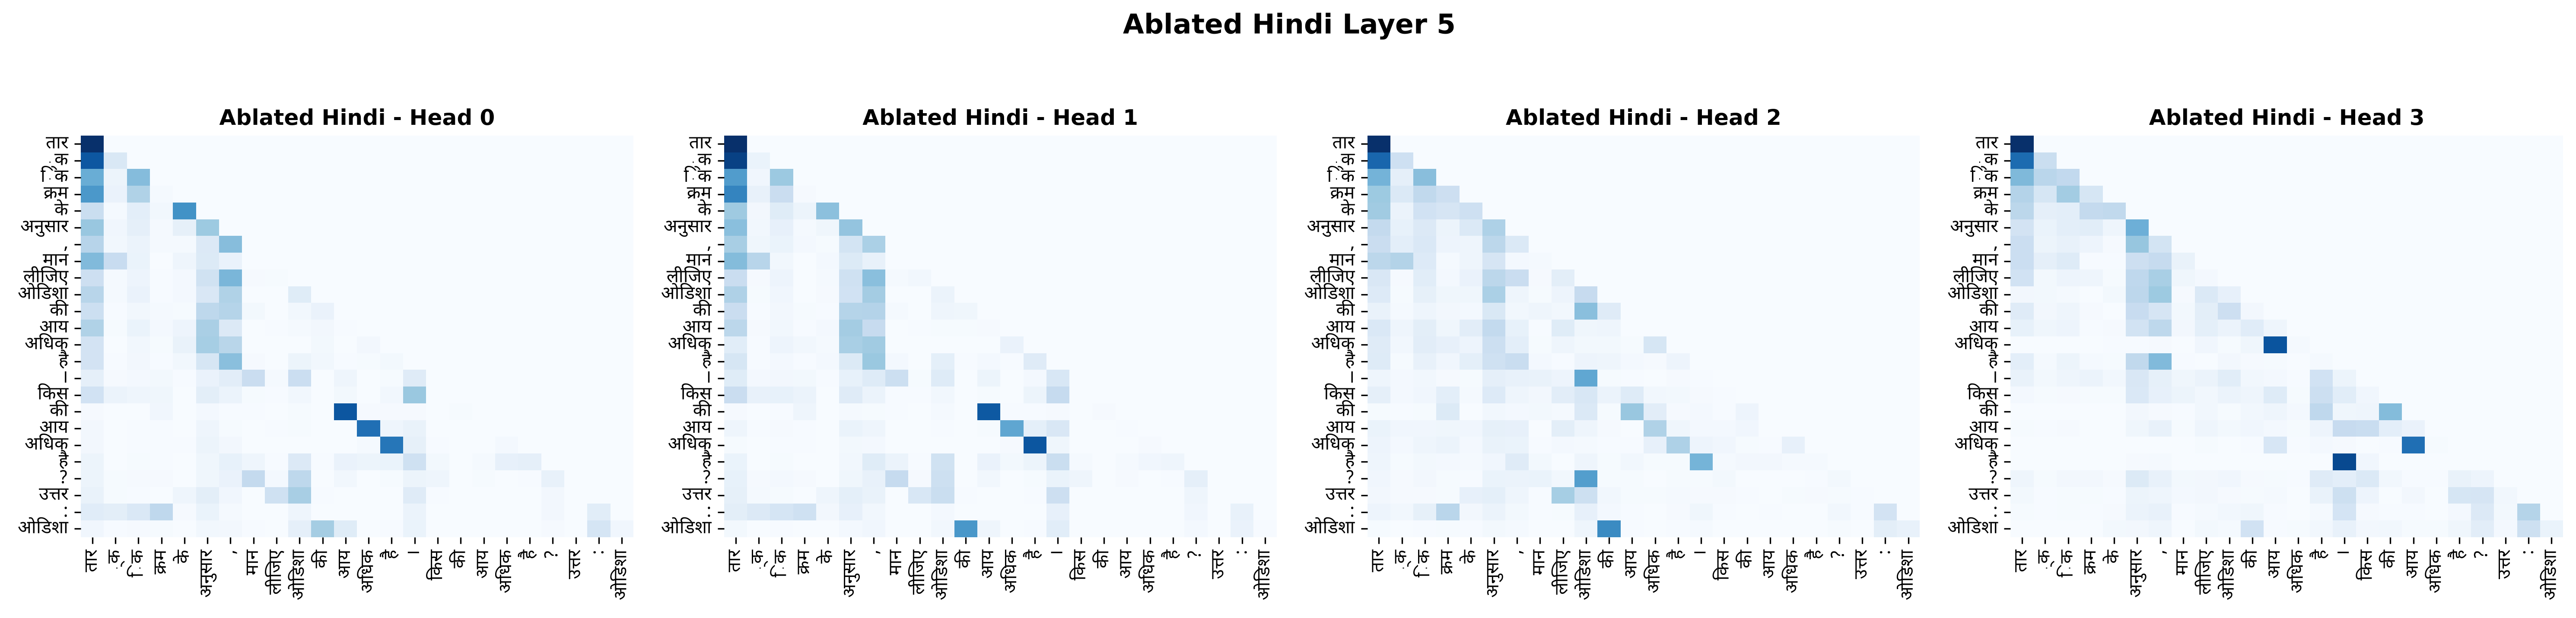
\includegraphics[width=\textwidth]{plots/bonus_ablation_attn_layer5.png}
  \caption{Ablated Hindi (No Pos-Emb): Layer 5 attention}
\end{subfigure}
\caption{Visual comparison of attention patterns between the Standard Model (with positional embeddings) and the Ablated Model (without positional embeddings). While the standard model learns rich contextual representations across layers, the ablated model collapses into a self-attending diagonal identity mapping, failing to establish relational context.}
\end{figure}

\begin{figure}[H]
\centering
\begin{subfigure}[b]{0.48\textwidth}
  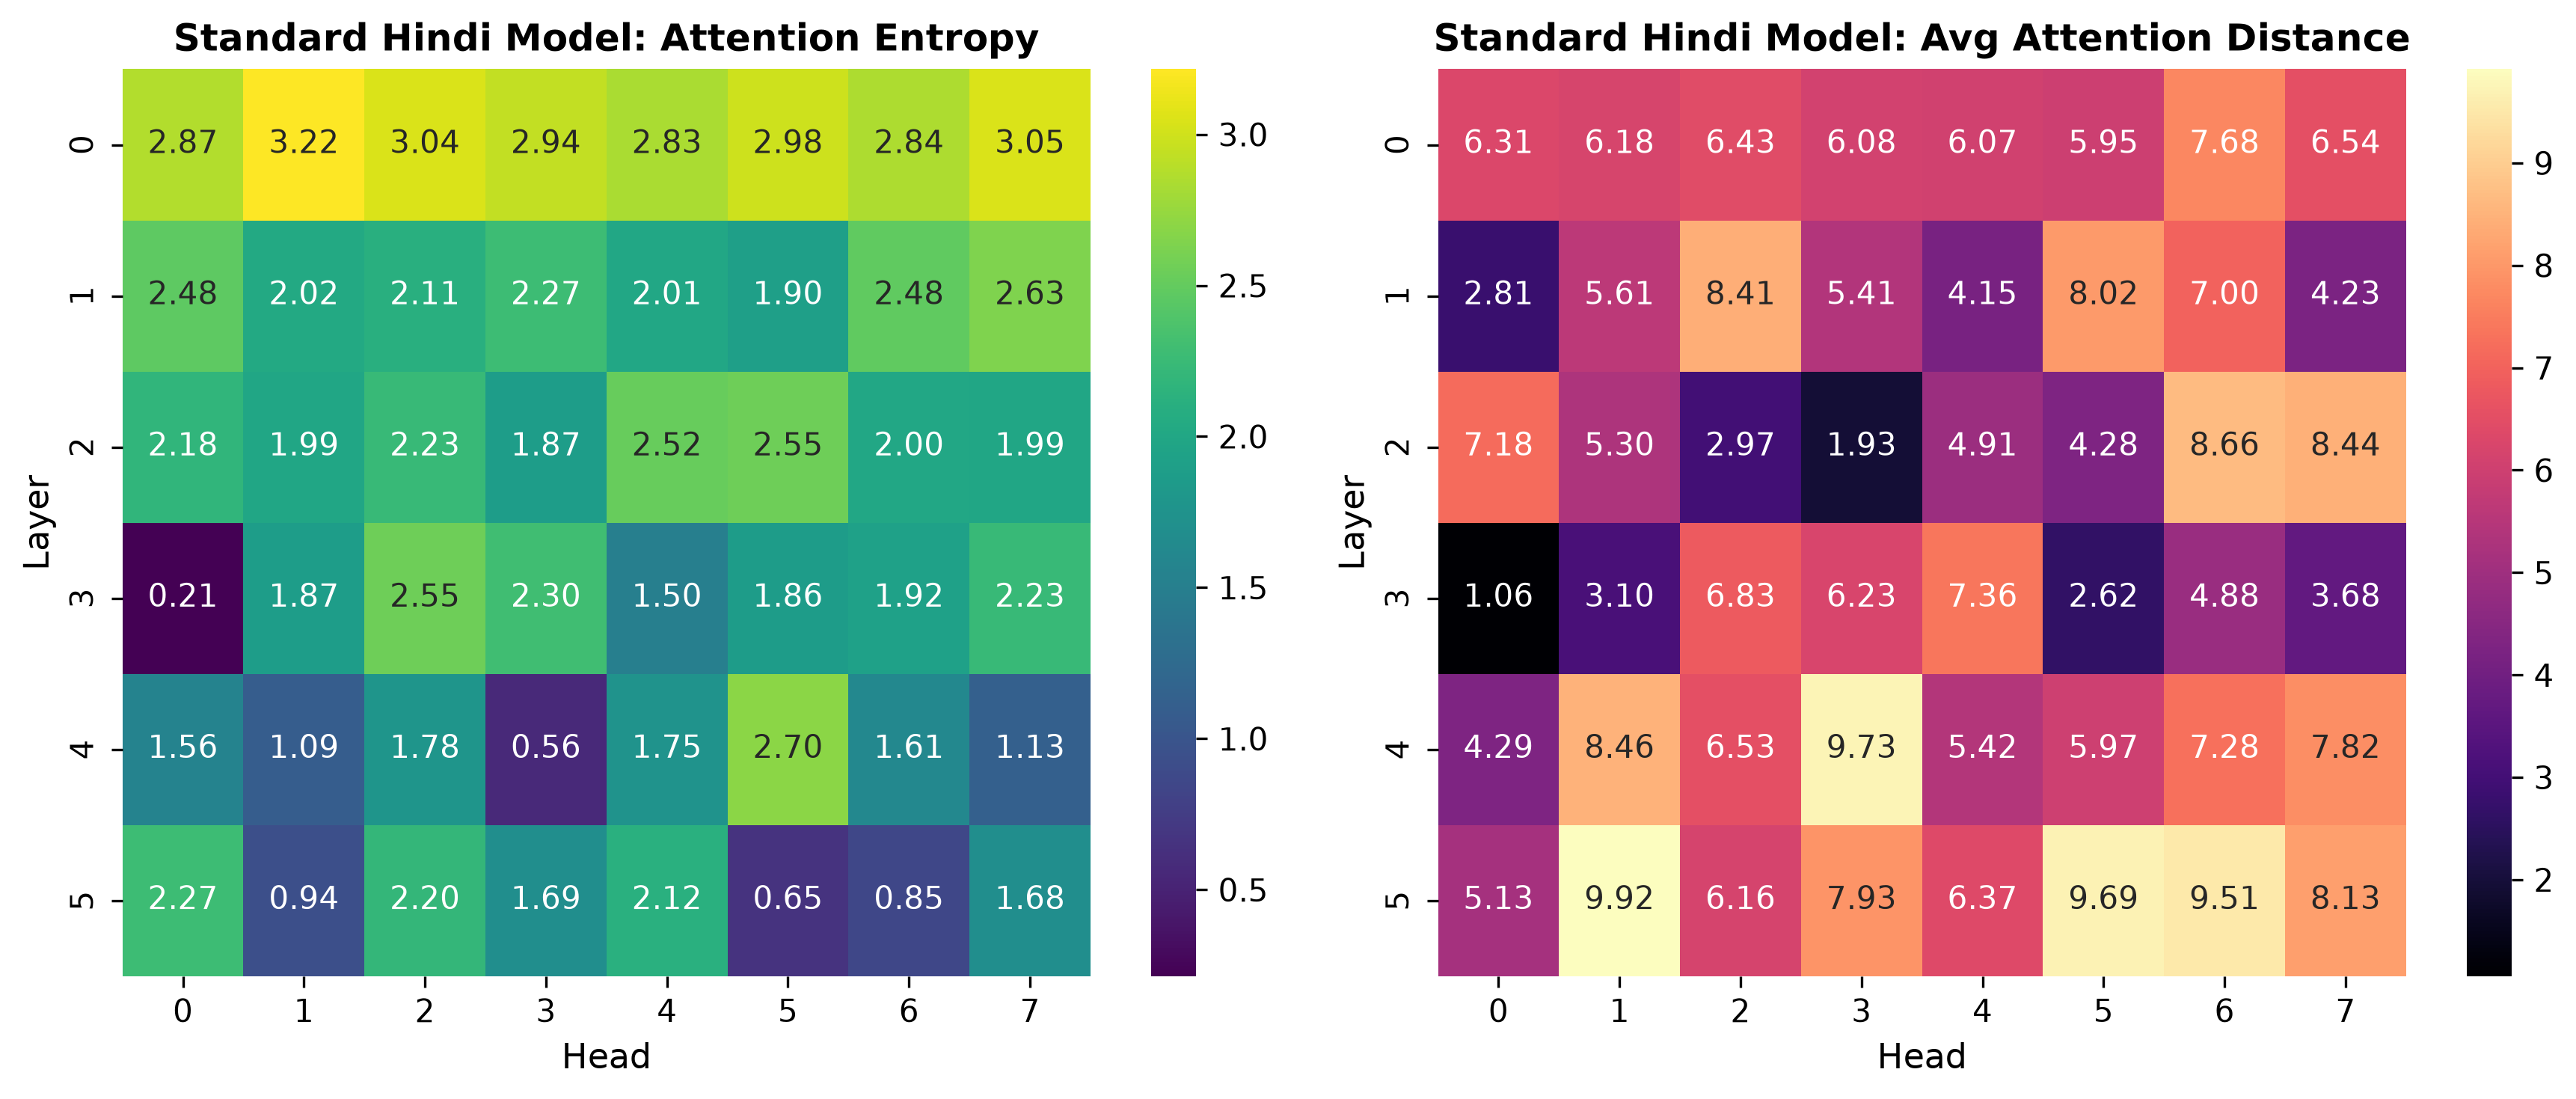
\includegraphics[width=\textwidth]{plots/phase2_hindi_attn_entropy_distance.png}
  \caption{Standard Model: Entropy \& Distance}
\end{subfigure}
\hfill
\begin{subfigure}[b]{0.48\textwidth}
  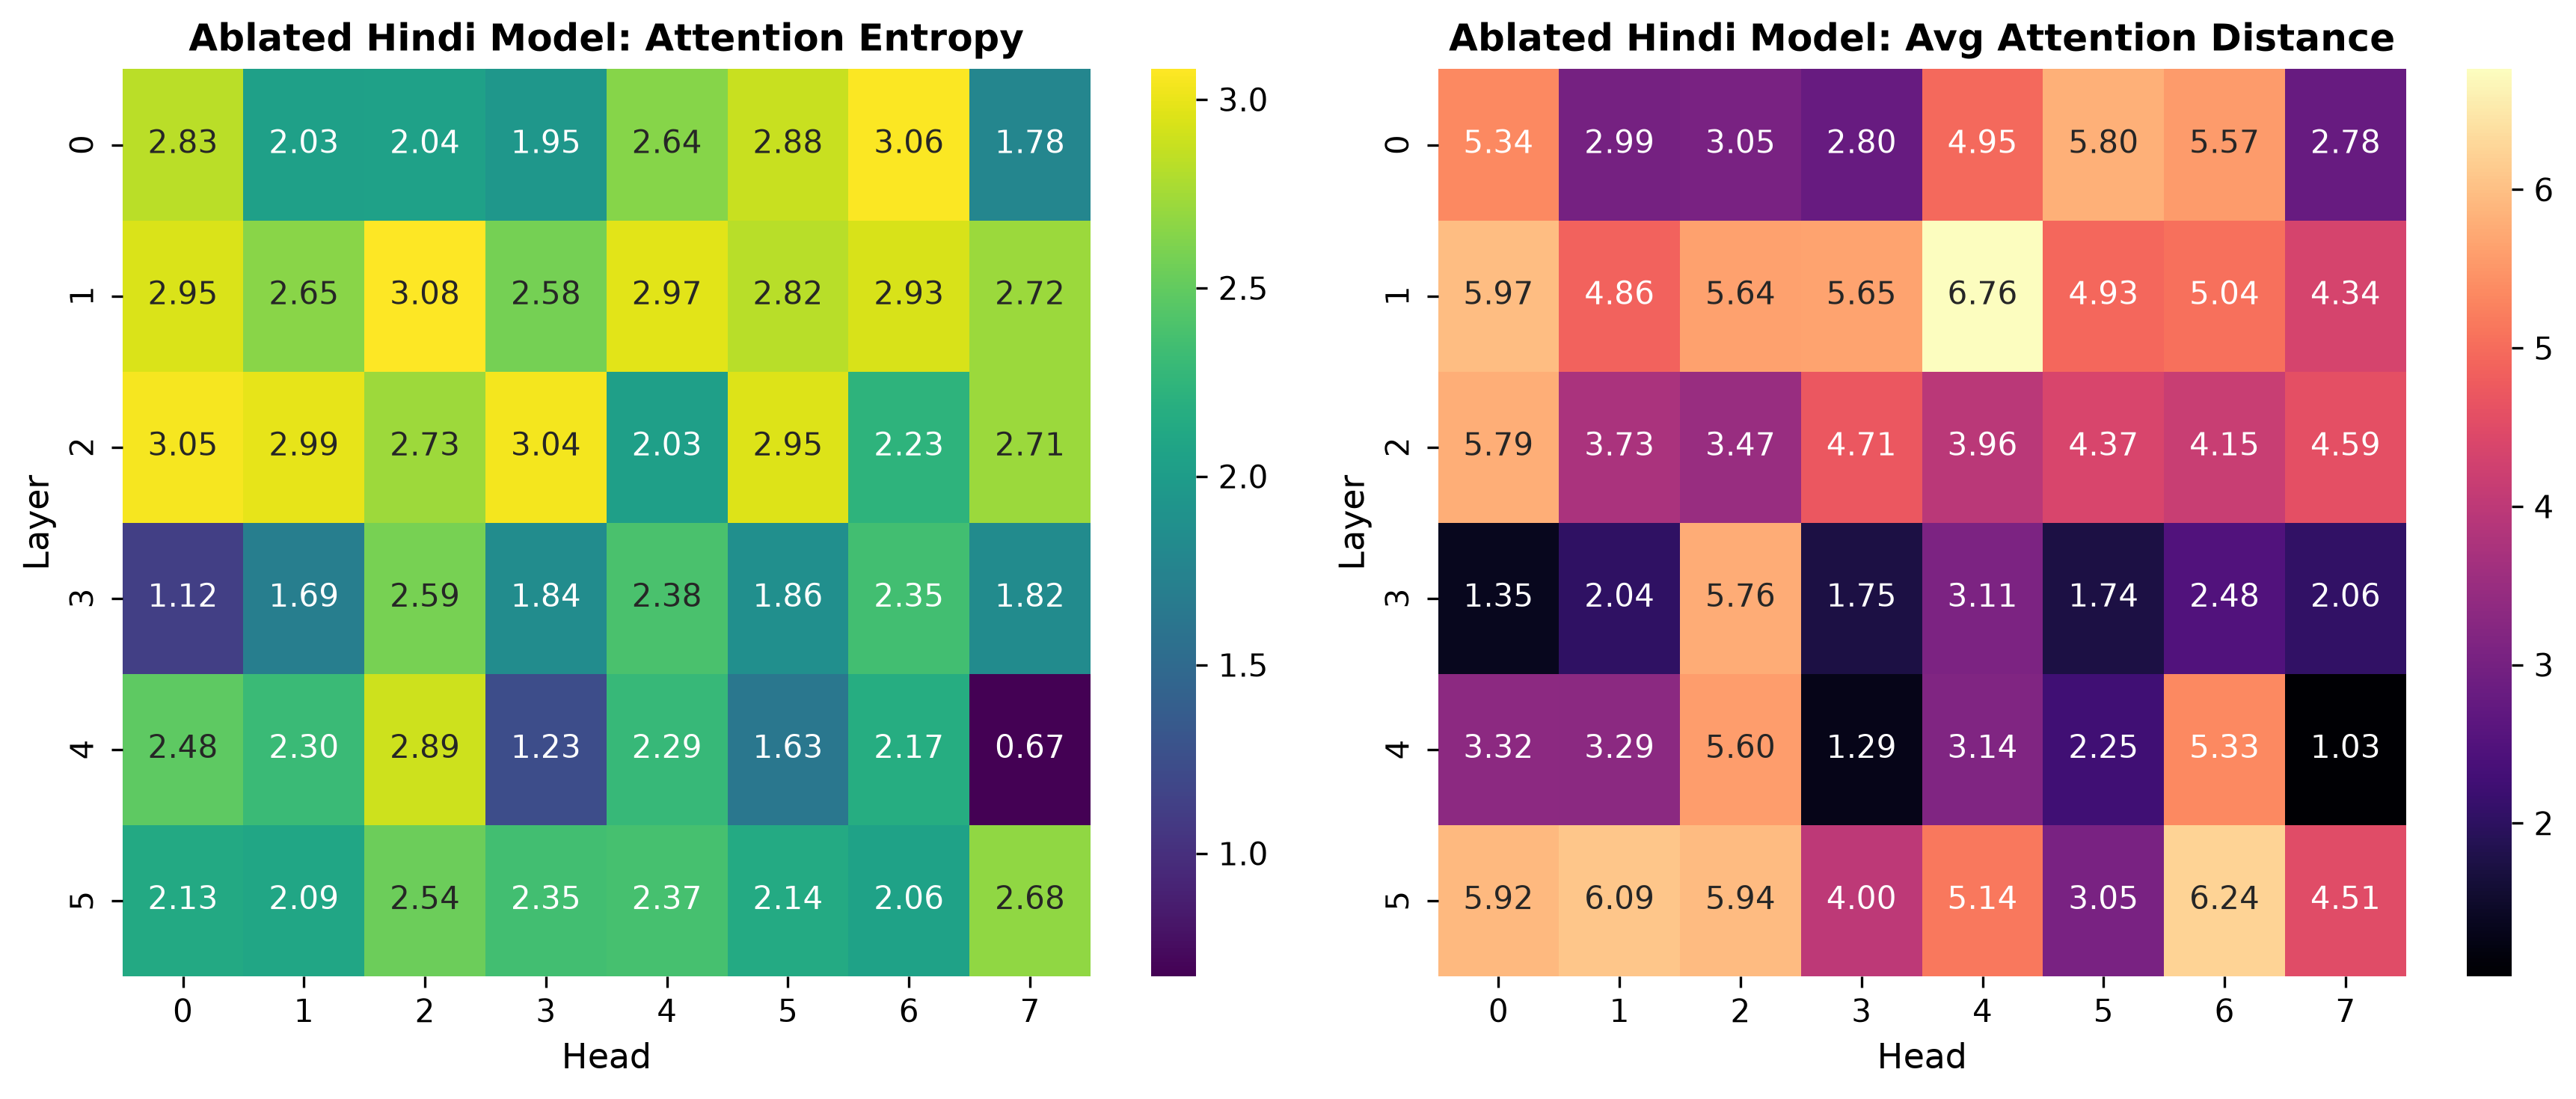
\includegraphics[width=\textwidth]{plots/bonus_ablation_attn_entropy_distance.png}
  \caption{Ablated Model: Entropy \& Distance}
\end{subfigure}
\caption{Entropy and mean attention distance across layers for Standard vs. Ablated models. The standard model exhibits distinct layer-wise functional specialization, whereas the ablated model demonstrates flattened metric profiles due to the lack of sequence order representation.}
\end{figure}

The standard model has clear structure: low-entropy local attention in early layers, higher-entropy long-range attention in later layers. The ablated model is flat across all layers, confirming the attention mechanism cannot organize itself without position information to anchor heads to.

% ===========================================================================
\section{Cross-Phase Comparison}

\subsection{Model H vs. Model L Summary}

\begin{table}[H]
\centering
\caption{Full Comparison Across Both Models and All Phases}
\small
\begin{tabular}{lccc}
\toprule
\textbf{Metric} & \textbf{Model H (Hindi)} & \textbf{Model L (Nepali)} & \textbf{Difference} \\
\midrule
\multicolumn{4}{l}{\textit{Phase 1: Tokenizer}} \\
Vocab Size & 16,000 & 16,240 & small \\
Bytes per Token & 10.31 & 13.16 & +27.6\% \\
\midrule
\multicolumn{4}{l}{\textit{Phase 2: Pretraining}} \\
Val Loss & 3.6487 & 3.5910 & Nepali better \\
Perplexity & 39.11 & 36.32 & Nepali better \\
BPB & 0.5131 & 0.3939 & Nepali better \\
Greedy 4-gram Rep. & 26.59\% & 67.12\% & Hindi much better \\
Distinct-1 (Greedy) & 0.4270 & 0.2291 & Hindi more diverse \\
\midrule
\multicolumn{4}{l}{\textit{Phase 3: Reasoning}} \\
Pretrained Baseline & 0.50\% & 2.00\% & near-identical \\
Finetuned Overall & 26.60\% & 25.20\% & near-identical \\
Tier 1 (Direct) & 39.68\% & 33.07\% & Hindi better \\
Tier 2 (Transitive) & 15.23\% & 15.45\% & identical \\
Tier 3 (Structural) & 37.29\% & 36.22\% & near-identical \\
\bottomrule
\end{tabular}
\end{table}

\subsection{Takeaways}

The most interesting outcome is how the two models compare at different phases. In Phase 2, Nepali actually wins on PPL and BPB because its tokenizer packs more bytes per token, but it loses badly on generation quality (67\% repetition rate vs 26\%). The tokenizer advantage is a compression artifact, not a real language modeling advantage.

In Phase 3, the two models are essentially tied at 26--27\% accuracy. The synthetic finetuning task equalizes both models by giving them the same number of examples with the same structure, removing the corpus breadth advantage Hindi has in Phase 2.

The conclusion is that for structured tasks with well-defined finetuning data, a lower-resource language can match a higher-resource one. The gap only appears in open-ended generation, where training corpus diversity directly limits output diversity.

% ===========================================================================
\section{Conclusion}

This project built two language models from scratch, covering the full pipeline from tokenizer training through pretraining to task-specific finetuning and ablation.

The main things learned:
\begin{itemize}
  \item Building attention from scratch with correct causal masking, shape handling, and positional embeddings is not trivial but gives complete visibility into what the model is doing.
  \item Lower-resource languages can match higher-resource ones on structured tasks if the finetuning data is designed carefully. The gap in pretraining corpus quality shows up in generation diversity, not in reasoning.
  \item Positional embeddings are not optional. Removing them completely breaks training, not just degrades it. The model loss never decreases.
  \item At 24M parameters with 6,300 finetuning examples, 27\% accuracy on multi-hop reasoning is near the fundamental representational limit of the model size.
\end{itemize}

All code, data, checkpoints, and evaluation scripts are available in the project repository and on Hugging Face (\texttt{manyajain111/LMA-Individual-Project}).

\end{document}

